\chapter{图的谱划分}
\label{chap:spectral-partition}

拉普拉斯矩阵零特征值的重数刻画图的连通分量个数。对于连通图，还可以进一步比较跨割边权与割两侧的规模，以识别连接较少的瓶颈并构造划分。

点连通度与边连通度对全图取最小，但不记录分隔后两侧的规模。等周数、导通率和比例割（RatioCut）引入了规模归一化，其一般情形的精确优化是NP难问题。谱方法把离散指示向量放宽为实向量，用特征值给出松弛下界，再沿相应谱坐标扫描候选割。后文将分别说明不同目标的下界、构造算法及其适用的性能保证。

本章记无向图的顶点集为$V$，边集为$E$，顶点数和边数分别为$n=|V|\geq 2$和$m=|E|$，边权非负，连通性按正权支撑判断。第~\ref{sec:graph-algebraic-connectivity}节从连通度的几何意义与不同连通度度量的对比出发，引入代数连通度$\lambda_2$与Fiedler向量$\bm v_2$；第~\ref{sec:graph-cheeger}节建立连接归一化谱$\mu_2$与最小导通率$\phi_*$的Cheeger不等式；第~\ref{sec:graph-ratiocut}至\ref{sec:graph-spectral-partition-comparison}节在此基础上系统展开RatioCut与NCut两种谱划分方法及其对比。

\section{代数连通度}
\label{sec:graph-algebraic-connectivity}

判断一张图是否连通，只需要检查任意两个顶点之间是否存在路径；但要刻画一张连通图“连得有多稳固”，则需要审视它的全局几何形态。本节先通过四类典型图建立“瓶颈”与“稀疏割”的几何图像，再对比局部组合连通度与全局稀疏割度量的局限，由此引出连续可算的代数连通度$\lambda_2$及其对应的Fiedler向量$\bm v_2$。

\subsection{连通度的几何意义}
\label{sec:graph-connectivity-geometry}

连通性只判断任意两点之间是否存在路径。对于已经连通的图，还可以考察删除多少条边会使它断开，以及断开后两侧的规模。图~\ref{fig:graph-connectivity-archetypes}通过四类图比较这些性质。

\begin{BookInlineFigure}
  \centering
  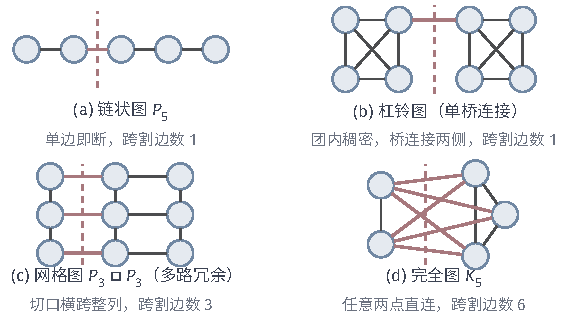
\includegraphics[width=96.238mm]{figures/03-graphs/05-matrices-and-spectra/tikz/connectivity-four-archetypes/figure.pdf}
  \caption{四类典型连通图的瓶颈结构对比。红色虚线标出将图切分为两个较大子集的最薄弱切口，红色实线为被切断的跨割边。(a) 链状图任一内边都是唯一通路；(b) 杠铃图两侧稠密但受制于中间的细腰单桥；(c) 网格图有多条平行通路，切口需横跨整列；(d) 完全图任意两部分之间都有密集边相连。}
  \label{fig:graph-connectivity-archetypes}
\end{BookInlineFigure}

第一类是\emph{链状图}（路径图$P_n$，$n\geq2$）。任意两点之间只有一条路径；删除任意一条边，或在$n\geq3$时删除任意内部顶点，都会使图分为两个连通分量。

第二类是\emph{杠铃图}（barbell graph）。这里取两个完全子图通过一条桥边相连的形式。两个子图内部均有较多连接，但删除中间的桥边就会使两侧断开。因此，局部边数较多并不保证全图没有规模较大的稀疏割。

第三类是\emph{网格图}$P_m\square P_m$（$m\geq2$）。它有$n=m^2$个顶点，每个内部顶点有四个邻居。沿相邻两列之间切开需要删除$m$条边；当$m$为偶数且从中间切开时，两侧顶点数相等。这个例子说明，某些图的均衡切分需要切断随规模增长的多条边。

第四类是\emph{完全图}$K_n$。将顶点集分成大小为$s$和$n-s$的两部分时，割边数为$s(n-s)$。当两侧大小都与$n$同阶时，割边数为$\Theta(n^2)$；若只隔离一个顶点，则只需删除$n-1$条边。讨论切分代价时，需要同时说明两侧的规模。

这些例子提示我们用\emph{稀疏割}（sparse cut）描述图中的连接瓶颈。对非空真子集$S\subsetneq V$，跨割边权为$c(S,\bar S)=\sum_{i\in S,j\in\bar S}w_{i,j}$。只有将它与两侧规模比较，才能区分“隔离一个低度顶点”和“分开两个较大的子图”。后面分别用顶点数与度数总和衡量规模，得到不同的稀疏割指标。

\subsection{连通度的度量}
\label{sec:graph-connectivity-measures}

如何将上述“瓶颈/稀疏割”的几何直觉转化为精确的数学度量？传统图论与组合优化分别从“最弱局部脱节代价”和“全局归一化割代价”两个角度提出了不同的指标，但二者在刻画能力与计算复杂度上各自面临根本困难。

\paragraph{局部组合连通度：$\kappa(\mathcal G)$、$\lambda(\mathcal G)$与$\delta(\mathcal G)$}

在经典图论中，简单无权图$\mathcal G=(V,E)$的连通程度通常由三个离散组合量来度量。第一个量是\term{点连通度}（vertex connectivity）$\kappa(\mathcal G)$，定义为使图变得不连通（或缩为单个顶点）所需删去的最少顶点数。第二个量是\term{边连通度}（edge connectivity）$\lambda(\mathcal G)$，定义为使图变得不连通所需删去的最少边数，即所有非空真子集割的最小割边数：
\begin{equation}
\label{eq:graph-edge-connectivity-def}
  \lambda(\mathcal G) = \min_{\varnothing\neq S\subsetneq V} c(S,\bar S).
\end{equation}
（注意此处带括号的$\lambda(\mathcal G)$表示图$\mathcal G$的边连通度，勿与带下标的拉普拉斯特征值$\lambda_1\leq\lambda_2\leq\cdots\leq\lambda_n$混淆。）第三个量是全图的\term{最小度数}（minimum degree）$\delta(\mathcal G)=\min_{v\in V}d_v$。

对任意顶点$v\in V$，只要删去与$v$关联的全部$d_v$条边，就能将单点$\{v\}$与其余顶点彻底隔开，因此必有$\lambda(\mathcal G)\leq\delta(\mathcal G)$；进一步，从最小边割的每条跨边中适当选取端点删去，又可证明$\kappa(\mathcal G)\leq\lambda(\mathcal G)$（详见定理~\ref{thm:graph-connectivity-comparison}）。三者满足经典的Whitney不等式：
\begin{equation}
\label{eq:graph-whitney-inequality}
  \kappa(\mathcal G) \leq \lambda(\mathcal G) \leq \delta(\mathcal G).
\end{equation}

点连通度$\kappa(\mathcal G)$与边连通度$\lambda(\mathcal G)$都是对全图取最小得到的量，但不记录最小分隔造成的两侧规模。图~\ref{fig:graph-connectivity-local-vs-global}中，$K_5$外接一个叶子与两个$K_4$经单桥相连的图均满足$\kappa=\lambda=1$；前者的最小边割隔离一个顶点，后者则把图分成等大的两部分。这两个指标本身不能区分这两种切分。

\begin{BookInlineFigure}
  \centering
  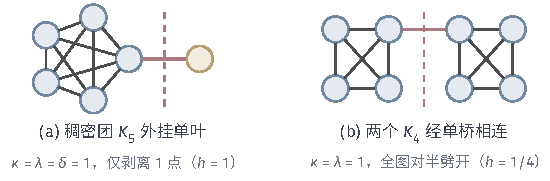
\includegraphics[width=93.059mm]{figures/03-graphs/05-matrices-and-spectra/tikz/connectivity-local-vs-global/figure.pdf}
  \caption{点、边连通度$\kappa(\mathcal G),\lambda(\mathcal G)$与等周数$h(\mathcal G)$的对比。(a) 稠密团$K_5$外挂单个叶子顶点，最弱局部切口仅剥离$1$个末梢顶点；(b) 两个$K_4$经单条桥边相连，最弱切口将全图对半劈开。两张图的$\kappa(\mathcal G)=\lambda(\mathcal G)=1$完全相同，但全局等周数分别为$h=1$与$h=1/4$。}
  \label{fig:graph-connectivity-local-vs-global}
\end{BookInlineFigure}

上述无权连通度只依赖边是否存在，不反映已有边的权重变化。若要比较加权网络，还需要采用割权或谱量。加权最小割值是若干线性函数的最小值，随边权连续变化，但在最优割改变时可能不可微；代数连通度也可能在特征值重合处不可微，因此连续性与可微性应分别讨论。

\paragraph{全局稀疏割指标与NP-Hard计算困境}

为了真正捕捉全局瓶颈，必须在跨割边代价$c(S,\bar S)$的分母上除以两侧子集的规模，迫使指标同时兼顾“割边少”与“两侧大”。按顶点数衡量集合规模时，最自然的全局稀疏割指标是图的\term{等周数}（isoperimetric number，亦称\term{Cheeger常数}）：
\begin{equation}
\label{eq:graph-isoperimetric-number}
  h(\mathcal G) = \min_{\varnothing\neq S\subsetneq V} \frac{c(S,\bar S)}{\min\{|S|,|\bar S|\}},
\end{equation}
以及对称兼顾两侧顶点数的\term{比例割}（RatioCut）：
\begin{equation}
\label{eq:graph-ratiocut-preview}
  \operatorname{RatioCut}(S) = c(S,\bar S)\left(\frac{1}{|S|}+\frac{1}{|\bar S|}\right).
\end{equation}
若改按度数总和（集合体积$\operatorname{vol}(S)=\sum_{i\in S}d_i$）衡量规模，则得到第~\ref{sec:graph-cheeger}节将深入研究的导通率$\phi(S)$与第~\ref{sec:graph-ncut}节的归一化割$\operatorname{NCut}(S)$。

在图~\ref{fig:graph-connectivity-local-vs-global}中，图(a)切下单叶时$\min\{|S|,|\bar S|\}=1$，等周数$h(\mathcal G)=1/1=1$；而图(b)沿桥边对半切开时$\min\{|S|,|\bar S|\}=4$，等周数为$h(\mathcal G)=1/4$，反映了两侧规模不同所带来的指标差异。

然而，这种全局精准性付出了高昂的计算代价：在包含$n$个顶点的图上，非空无序二分共有$2^{n-1}-1$种；精确求解最小等周数$h(\mathcal G)$、最小导通率$\phi_*$或最小RatioCut，均已被证明是\emph{NP-Hard组合优化难题}。当图的顶点数达到数千乃至数百万时，遍历所有离散子集寻找最稀疏割在计算上完全不可行。

因此可以考虑连续松弛：用能够高效近似计算的特征值给出离散割目标的界，再从特征向量构造候选划分。

\subsection{代数连通度}
\label{sec:graph-algebraic-connectivity-variational}

这个连续可算替代品正是组合拉普拉斯矩阵$\bm L=\bm D-\bm W$的第二小特征值$\lambda_2$。为了理解$\lambda_2$为何能度量全局连通程度，我们先从拉普拉斯二次型的沿边能量出发给出它的定义与变分刻画，再证明它与经典连通度及全局稀疏割的定量关系。

\paragraph{代数连通度的定义与变分刻画}

回顾第~\ref{sec:graph-laplacian-energy}节，给每个顶点$i$赋予实数值$x_i$时，组合拉普拉斯二次型
\[
  \bm x^\top\bm L\bm x = \sum_{\{i,j\}\in E} w_{i,j}(x_i-x_j)^2
\]
累加了所有边两端读数差的平方，衡量向量$\bm x$在图上的沿边变化能量。例如在图~\ref{fig:graph-partition-edge-energy}(a)的单位权四点路径上，给前两个顶点赋$+1$、后两个赋$-1$，只有中间边$23$产生差值$1-(-1)=2$，总能量为$4$；而在图~\ref{fig:graph-partition-edge-energy}(b)中添入跨接首尾的边$14$后，同一赋值的总能量增至$8$。

\begin{BookInlineFigure}
  \centering
  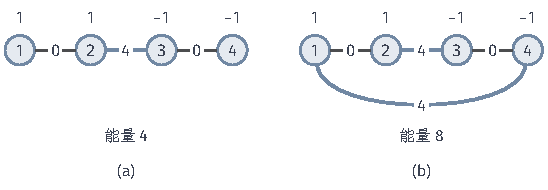
\includegraphics{figures/03-graphs/05-matrices-and-spectra/tikz/partition-edge-energy/figure.pdf}
  \caption{对同一组顶点赋值计算沿边能量。(a) 四点路径，只有中间边贡献了能量$4$。(b) 加上边$14$后得到四边环，新增的边上也有差$2$，总能量变为$8$。顶点上方是赋值，边上的数是差的平方。}
  \label{fig:graph-partition-edge-energy}
\end{BookInlineFigure}

要在给定图上寻找“沿边能量最小”的非平凡顶点赋值，必须满足两条规范化约束。第一，给所有顶点赋相同的常数时，每条边两端差均为零，能量恒为零；这种常值赋值不反映任何图结构信息，因此需要要求赋值向量与全一常向量正交，即满足零和条件$\bm x\perp\bm 1$（$\sum_{i=1}^n x_i=0$）。

第二，将非零向量$\bm x$同乘常数$c\neq 0$会使能量$\bm x^\top\bm L\bm x$与欧氏长度平方$\bm x^\top\bm x$同步放大$c^2$倍；为了在同一尺度下公平比较不同方向，应当考察两者的比值——即Rayleigh商$\frac{\bm x^\top\bm L\bm x}{\bm x^\top\bm x}$。Fiedler于1973年提出将非平凡方向上的最小Rayleigh商定义为图的代数连通度。

\begin{definition}[代数连通度]
\label{def:graph-algebraic-connectivity}
设$n$阶无向非负加权图$\mathcal G$的组合拉普拉斯矩阵$\bm L$的特征值按升序排列为$0=\lambda_1\leq\lambda_2\leq\cdots\leq\lambda_n$。图的\term{代数连通度}（algebraic connectivity）定义为第二小特征值$\lambda_2(\mathcal G)$（在不致混淆时简记为$\lambda_2$），其Courant--Fischer变分刻画为
\begin{equation}
\label{eq:graph-algebraic-connectivity}
\lambda_2
=\min_{\substack{\bm x\perp\bm 1\\\bm x\ne\bm 0}}
\frac{\bm x^\top\bm L\bm x}{\bm x^\top\bm x}
=\min_{\substack{\bm x^\top\bm 1=0\\\lVert\bm x\rVert_2=1}}
\bm x^\top\bm L\bm x.
\end{equation}
\end{definition}

将式~\eqref{eq:graph-algebraic-connectivity}与前文的正交特征展开相对照，可以一步看清该极小值的代数结构。设$\bm v_1=\bm 1/\sqrt{n},\bm v_2,\ldots,\bm v_n$为$\bm L$对应于$0=\lambda_1\leq\lambda_2\leq\cdots\leq\lambda_n$的标准正交特征向量基。

任取满足$\bm x\perp\bm 1$的非零向量$\bm x$，它在$\bm v_1$方向上的投影系数为零，故可展开为$\bm x=\sum_{k=2}^n\alpha_k\bm v_k$。

代入Rayleigh商并利用特征向量的正交性，可得
\[
  \frac{\bm x^\top\bm L\bm x}{\bm x^\top\bm x}
  = \frac{\sum_{k=2}^n\lambda_k\alpha_k^2}{\sum_{k=2}^n\alpha_k^2}
  \geq \lambda_2,
\]
且当$\bm x$取为$\lambda_2$对应的特征向量$\bm v_2$时等号精确成立。

由这一变分刻画立即可读出代数连通度的三项基本性质：
\begin{enumerate}
\item \emph{连通性的充要判据}：由第~\ref{sec:graph-laplacian-kernel}小节知，$\bm L$的零特征值重数等于图$\mathcal G$的连通分量个数。因此$\lambda_2>0$当且仅当$\mathcal G$连通；$\lambda_2=0$当且仅当$\mathcal G$不连通。
\item \emph{关于边权与加边的单调性}：若在相同顶点集上增大边权或添加新边得到$\mathcal G'$，则对每个零和向量$\bm x$都有$\bm x^\top\bm L(\mathcal G')\bm x\geq\bm x^\top\bm L(\mathcal G)\bm x$，取最小后即得$\lambda_2(\mathcal G')\geq\lambda_2(\mathcal G)$。
\item \emph{典型图族的定量对比}：结合第~\ref{sec:graph-typical-laplacian-spectra}小节算出的典型图谱，四类典型图（图~\ref{fig:graph-connectivity-archetypes}）的代数连通度呈现出鲜明的量级差异：链状路径图$\lambda_2(P_n)=2\bigl(1-\cos(\pi/n)\bigr)=\Theta(n^{-2})$，随$n$增大迅速衰减至$0$；由两个$K_m$经单桥相连的杠铃图（$m\geq2$，$n=2m$）满足$\lambda_2=\bigl(m+2-\sqrt{(m+2)^2-8}\bigr)/2=\Theta(m^{-1})=\Theta(n^{-1})$，定量暴露出细腰瓶颈；二维网格图$\lambda_2(P_m\square P_m)=2\bigl(1-\cos(\pi/m)\bigr)=\Theta(n^{-1})$，比链状图高出一个量级；而完全图$\lambda_2(K_n)=n$随规模线性增长，成为所有$n$阶简单无权图的上界。
\end{enumerate}

\paragraph{代数连通度与其他连通度的关系}

代数连通度$\lambda_2$不仅在定性趋势上区分了不同图族，而且与前文介绍的局部组合连通度$\kappa(\mathcal G),\lambda(\mathcal G),\delta(\mathcal G)$以及全局稀疏割指标$h(\mathcal G),\operatorname{RatioCut}$之间存在严格的不等式联系。我们先证明Fiedler关于局部连通度的经典上界定理。

\begin{theorem}[代数连通度与点、边连通度的比较]
\label{thm:graph-connectivity-comparison}
设$\mathcal G=(V,E)$为有限简单无权连通非完全图，则其代数连通度$\lambda_2(\mathcal G)$、点连通度$\kappa(\mathcal G)$、边连通度$\lambda(\mathcal G)$与最小度数$\delta(\mathcal G)$满足
\begin{equation}
\label{eq:graph-connectivity-comparison}
  \lambda_2(\mathcal G)\leq\kappa(\mathcal G)\leq\lambda(\mathcal G)\leq\delta(\mathcal G).
\end{equation}
\end{theorem}

\begin{proof}
我们按从左到右的顺序分三步证明式~\eqref{eq:graph-connectivity-comparison}中的三个不等号。

第一步：证明$\lambda_2(\mathcal G)\leq\kappa(\mathcal G)$。因为$\mathcal G$是连通非完全图，必存在最小点分隔集$T\subsetneq V$（$|T|=\kappa(\mathcal G)$），使得删去$T$后剩余顶点集$V\setminus T$至少分裂为两个互不相连的非空部分。取其中一个连通块记为$A$，将其余所有块合并记为$B=V\setminus(T\cup A)$，则$A,B$均非空，且$A$与$B$之间没有任何直接边相连。

构造如下三值试探向量$\bm x\in\mathbb R^n$：对$i\in A$令$x_i=|B|$，对$i\in B$令$x_i=-|A|$，对$i\in T$令$x_i=0$。

核对零和条件：$\bm x$的各分量之和为
\[
  \sum_{i=1}^n x_i = |A|\cdot|B| + |B|\cdot(-|A|) + |T|\cdot 0 = 0,
\]
故$\bm x\perp\bm 1$且$\bm x\neq\bm 0$。

计算分母的欧氏长度平方：
\[
  \bm x^\top\bm x = |A|\cdot|B|^2 + |B|\cdot|A|^2 = |A||B|(|A|+|B|).
\]

计算分子的沿边能量$\bm x^\top\bm L\bm x$：$A$内部各点取值恒为$|B|$，差为零；$B$内部各点取值恒为$-|A|$，差为零；$T$内部各点取值恒为$0$，差也为零；而$A$与$B$之间无边。因此，只有一端在$T$、另一端在$A$或$B$的边才对能量有贡献。

由于$\mathcal G$是简单无权图，$A$中的每个顶点至多与$T$中的$|T|$个顶点相邻，每条这样的边贡献$(|B|-0)^2=|B|^2$；同理，$B$中的每个顶点至多与$T$中的$|T|$个顶点相邻，每条这样的边贡献$(-|A|-0)^2=|A|^2$。累加可得分子上界：
\[
  \bm x^\top\bm L\bm x
  \leq |T|\bigl(|A|\cdot|B|^2 + |B|\cdot|A|^2\bigr)
  = |T|\cdot|A||B|(|A|+|B|).
\]

将分子上界除以分母$\bm x^\top\bm x$，结合变分刻画式~\eqref{eq:graph-algebraic-connectivity}即得
\[
  \lambda_2(\mathcal G)\leq\frac{\bm x^\top\bm L\bm x}{\bm x^\top\bm x}\leq |T|=\kappa(\mathcal G).
\]

第二步：证明$\kappa(\mathcal G)\leq\lambda(\mathcal G)$。取一个大小为$\lambda(\mathcal G)$的最小边割$c(S,\bar S)$。若在两侧能找到一对不相邻的顶点$u\in S$与$v\in\bar S$，则每条跨割边至少有一个端点不属于$\{u,v\}$；从每条跨割边各选一个异于$u,v$的端点组成集合$T$，则$|T|\leq\lambda(\mathcal G)$且删去$T$即切断了$u$与$v$之间的所有跨边，故$\kappa(\mathcal G)\leq|T|\leq\lambda(\mathcal G)$。

若$S$与$\bar S$之间的所有可能边都存在，设$|S|=p,|\bar S|=q$，则$\lambda(\mathcal G)=pq$；由$(p-1)(q-1)\geq 0$知$pq\geq p+q-1=n-1$，而在非完全图中任取一对不相邻顶点并删去其余$n-2$个顶点即可断开图，故仍有$\kappa(\mathcal G)\leq n-2<n-1\leq\lambda(\mathcal G)$。

第三步：证明$\lambda(\mathcal G)\leq\delta(\mathcal G)$。取达到最小度数的顶点$v_0$（$d_{v_0}=\delta(\mathcal G)$），令$S=\{v_0\}$，则割$(S,\bar S)$恰好切断与$v_0$关联的$\delta(\mathcal G)$条边，故$\lambda(\mathcal G)\leq c(\{v_0\},V\setminus\{v_0\})=\delta(\mathcal G)$。
\end{proof}

在单位权四点路径$P_4$上，$\lambda_2=2-\sqrt 2\approx 0.586<\kappa(P_4)=\lambda(P_4)=\delta(P_4)=1$；在四元环$C_4$上，$\lambda_2=\kappa(C_4)=\lambda(C_4)=\delta(C_4)=2$，不等式链全部取等（图~\ref{fig:graph-connectivity-separator-trial}）。完全图$K_n$之所以在定理~\ref{thm:graph-connectivity-comparison}中单独排除，是因为$K_n$中不存在不相邻的顶点对，无法删点将其分成两个不相连的非空部分，按约定$\kappa(K_n)=\lambda(K_n)=\delta(K_n)=n-1$，而$\lambda_2(K_n)=n$。

\begin{BookInlineFigure}
  \centering
  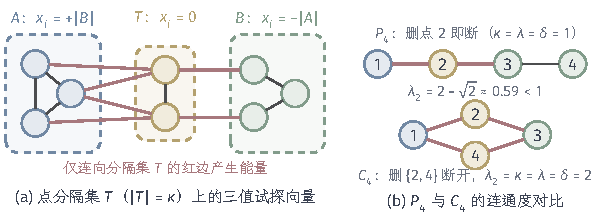
\includegraphics[width=102.164mm]{figures/03-graphs/05-matrices-and-spectra/tikz/connectivity-separator-trial/figure.pdf}
  \caption{点分隔集试探向量构造与连通度不等式核对。(a) 删去最小点分隔集$T$（$|T|=\kappa$）将图分为互不相连的$A$与$B$；给$A$赋$+|B|$、$B$赋$-|A|$、$T$赋$0$后，仅连向$T$的红边产生沿边能量。(b) $P_4$（严格不等式）与$C_4$（等号成立）的连通度对比。}
  \label{fig:graph-connectivity-separator-trial}
\end{BookInlineFigure}

除了受局部连通度$\kappa(\mathcal G)$上界控制之外，代数连通度$\lambda_2$还直接给出了全局等周数$h(\mathcal G)$与最小RatioCut的\emph{连续下界}。对任意非空真子集$S\subsetneq V$（记$s=|S|,t=|\bar S|=n-s$），在式~\eqref{eq:graph-algebraic-connectivity}中代入中心化两值试探向量$\bm y=\bm 1_S-\frac{s}{n}\bm 1$（详见第~\ref{sec:graph-ratiocut-relaxation}小节定理~\ref{prop:graph-ratiocut-relaxation}），立即可得
\begin{equation}
\label{eq:algebraic-connectivity-isoperimetric-bound}
  \lambda_2(\mathcal G)
  \leq \frac{\bm y^\top\bm L\bm y}{\bm y^\top\bm y}
  = c(S,\bar S)\left(\frac{1}{|S|}+\frac{1}{|\bar S|}\right)
  = \operatorname{RatioCut}(S)
  \leq \frac{2\,c(S,\bar S)}{\min\{|S|,|\bar S|\}}.
\end{equation}
对所有非空真子集$S$取最小后，即得全局稀疏割的下界关系：
\begin{equation}
\label{eq:algebraic-connectivity-cheeger-lower}
  \frac{\lambda_2(\mathcal G)}{2}
  \leq \frac{1}{2}\min_{\varnothing\neq S\subsetneq V}\operatorname{RatioCut}(S)
  \leq h(\mathcal G).
\end{equation}
式~\eqref{eq:algebraic-connectivity-cheeger-lower}给出了按顶点数归一化的割权下界：$h(\mathcal G)\geq\lambda_2/2$。这里的尺度仍依赖边权；把全部边权同乘常数会使$\lambda_2$和$h$同比变化。若希望指标对这种整体缩放不变，可以改用度加权体积作分母，这将引出下一节的导通率与归一化拉普拉斯。

\subsection{Fiedler向量}
\label{sec:graph-fiedler-vector}

代数连通度$\lambda_2$给出割权的谱下界，而相应的特征向量$\bm v_2$提供一维顶点坐标，可据此构造候选划分。它一般不直接给出最优稀疏割。

\begin{definition}[Fiedler向量]
\label{def:graph-fiedler-vector}
设连通无向非负加权图$\mathcal G$的组合拉普拉斯矩阵为$\bm L$。对应于代数连通度$\lambda_2>0$的非零特征向量$\bm v_2$（即满足$\bm L\bm v_2=\lambda_2\bm v_2$且$\bm v_2^\top\bm 1=0$，亦常记作$\bm f$）称为图的\term{Fiedler向量}（Fiedler vector）。
\end{definition}

如果$\lambda_2$是单重特征值，单位长度的Fiedler向量在差一个正负号的意义下唯一确定；若$\lambda_2$为重根，则对应的特征子空间中任意非零向量都是Fiedler向量。由于连通图上$\bm v_2\perp\bm 1$，Fiedler向量的所有分量之和为零：$\sum_{i=1}^n(\bm v_2)_i=0$，因此它必然同时包含正分量与负分量。

\paragraph{Fiedler向量$\bm v_2$的物理与几何意义}

我们可以从弹簧势能、振动和扩散三个角度理解$\bm v_2$为何可用于构造划分。

第一个视角是\emph{一维胡克弹簧网络的最小势能嵌入}。将图中的每条边$\{i,j\}$看作劲度系数为$w_{i,j}$的理想弹簧，把每个顶点$i$放置在实数轴上的坐标$x_i=(\bm v_2)_i$处，则拉普拉斯二次型的一半$\frac12\bm x^\top\bm L\bm x=\frac12\sum_{\{i,j\}\in E}w_{i,j}(x_i-x_j)^2$恰好是整个弹簧系统的总弹性势能。零和条件$\sum_i x_i=0$将全部顶点的重心固定在原点$0$，单位长度条件$\sum_i x_i^2=1$则固定了顶点在实轴上的总展开尺度，防止所有顶点坍缩到原点以逃避势能。

在零和与单位长度约束下，最小化Rayleigh商等价于最小化上述弹簧势能。图~\ref{fig:graph-fiedler-barbell}中的两个三角形仅由边$3\!-\!4$连接，其Fiedler向量在两个三角形上分别取负值和正值，团内坐标差小于桥边两端的坐标差。这说明该图的低能量方向能够反映桥边所连接的两个部分；对于一般图，仍须计算各候选割的目标值来判断划分质量。

\begin{BookInlineFigure}
  \centering
  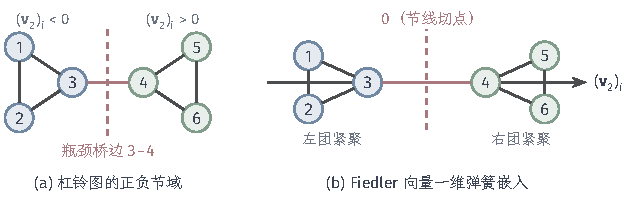
\includegraphics[width=107.495mm]{figures/03-graphs/05-matrices-and-spectra/tikz/fiedler-barbell-embedding/figure.pdf}
  \caption{杠铃图上Fiedler向量$\bm v_2$的物理意义与一维弹簧嵌入。(a) 两个三角形团$\{1,2,3\}$与$\{4,5,6\}$经单条瓶颈桥边$3\!-\!4$相连，$\bm v_2$在左团取负值、右团取正值；(b) 将顶点放置在实轴坐标$(\bm v_2)_i$上时，团内密集弹簧将各自顶点紧紧聚拢在两侧，唯一的瓶颈桥边被大幅拉伸并跨越原点$0$（红色虚线切点）。}
  \label{fig:graph-fiedler-barbell}
\end{BookInlineFigure}

第二个视角是\emph{弹性振动的基频驻波模态}。在质量均匀的离散振动网络$\frac{\mathrm d^2\bm u}{\mathrm dt^2}=-\bm L\bm u$中，$\lambda_1=0$对应全体顶点同向平移的刚体运动（零频模态），而$\lambda_2>0$对应的$\bm v_2$则是系统的第一阶非平凡简谐振动模态（基频驻波）。正负分量表示相反的振动相位，角频率为$\sqrt{\lambda_2}$。在上述杠铃图中，两团以相反相位振动；一般图的符号边界不保证对应最优稀疏割。

第三个视角是\emph{图上热扩散的最慢衰减模态}。在连续时间热传导或共识扩散方程$\frac{\mathrm d\bm x}{\mathrm dt}=-\bm L\bm x$中，任意初始温度分布$\bm x(0)=\sum_{k=1}^n\alpha_k\bm v_k$按$\bm x(t)=\alpha_1\bm v_1+\sum_{k=2}^n\alpha_k\mathrm e^{-\lambda_k t}\bm v_k$演化。非恒定模态按各自的$\mathrm e^{-\lambda_k t}$衰减，最小正特征值$\lambda_2$对应最慢衰减率。若$\lambda_2$为重特征值，整个对应特征子空间具有相同的衰减率；该部分是否出现在演化中，还取决于初值在此子空间上的投影。

\paragraph{Fiedler节域连通性定理}

按Fiedler向量的符号可以构造二分候选。下面的Fiedler节域连通性定理保证非负顶点集和非正顶点集各自诱导连通子图；这是一项连通性结论，不是割目标最优性的保证。

\begin{theorem}[Fiedler节域连通性定理]
\label{thm:graph-fiedler-connected-side}
设有限无向加权图$\mathcal G$的正权支撑连通，$\bm f=\bm v_2$为组合拉普拉斯矩阵$\bm L$的Fiedler向量。则非负顶点集合$V_+=\{i\in V:f_i\geq 0\}$（以及对称地，非正顶点集合$V_-=\{i\in V:f_i\leq 0\}$）所诱导的正权子图必定连通。
\end{theorem}

\begin{proof}
由$\bm f$与$-\bm f$的对称性，只需证明$V_+=\{i:f_i\geq 0\}$诱导的正权子图连通。反设$V_+$分裂成了两个或更多个互不连通的连通块，我们将导出矛盾。

第一步：写出单个非负连通块上的特征方程。记严格负值顶点集合为$N=\{j\in V:f_j<0\}$，任取$V_+$的一个连通块$C$。由于$V_+$的不同连通块之间没有正权边相连，特征方程$\bm L\bm f=\lambda_2\bm f$限制在块$C$的坐标上只涉及$C$自身与负值集$N$：
\[
  \bm L_{C,C}\bm f_C = \lambda_2\bm f_C - \bm r_C,
  \qquad
  \bm r_C = \bm L_{C,N}\bm f_N.
\]
矩阵块$\bm L_{C,N}$的元素为$-w_{i,j}\leq 0$（$i\in C,j\in N$），而$\bm f_N$的分量全部严格为负，故$\bm r_C$的每个分量$(\bm r_C)_i=\sum_{j\in N}w_{i,j}(-f_j)\geq 0$。又因原图连通且$C$不与$V_+\setminus C$相连，$C$至少有一条正权边连向$N$，从而$\bm r_C$是逐项非负且至少有一项严格为正的向量。

第二步：利用块主子矩阵的正Perron向量证明$\theta_C<\lambda_2$。取实数$a>0$足够大，使$\bm M_C=a\bm I-\bm L_{C,C}$逐项非负。因为$C$诱导的正权子图连通，沿用第~\ref{sec:adjacency-perron-theorem}节Perron定理的证明（对角非负项不影响取绝对值和沿正权边传播的论证，单点块可直接验证），$\bm M_C$的最大特征值对应的特征向量可取为分量全部严格为正的向量$\bm z>\bm 0$。若记$\theta_C$为对称块$\bm L_{C,C}$的最小特征值，则$a-\theta_C$正是$\bm M_C$的最大特征值，故$\bm L_{C,C}\bm z=\theta_C\bm z$。

将第一步的块方程左乘$\bm z^\top$，利用$\bm z^\top\bm L_{C,C}=\theta_C\bm z^\top$可得
\[
  \theta_C\,\bm z^\top\bm f_C
  = \lambda_2\,\bm z^\top\bm f_C - \bm z^\top\bm r_C.
\]
注意$\bm f_C\geq\bm 0$且不可能全为零（若$\bm f_C=\bm 0$，则由第一步方程得$\bm r_C=\bm 0$，与$\bm r_C$至少有一项为正矛盾）。结合$\bm z>\bm 0$可知$\bm z^\top\bm f_C>0$且$\bm z^\top\bm r_C>0$。两边同除以$\bm z^\top\bm f_C$即得
\[
  \theta_C = \lambda_2 - \frac{\bm z^\top\bm r_C}{\bm z^\top\bm f_C} < \lambda_2.
\]
这表明$V_+$的每一个连通块$C$的最小特征值$\theta_C$都严格小于$\lambda_2$。

第三步：由Cauchy交错定理导出矛盾。若$V_+$至少有两个连通块$C_1,C_2$，则$\bm L$在$V_+$上的主子矩阵$\bm L_{V_+,V_+}$是以各连通块$\bm L_{C_r,C_r}$为对角块的分块对角矩阵，其全体特征值是各块特征值的并集。由于$\theta_{C_1}<\lambda_2$且$\theta_{C_2}<\lambda_2$，主子矩阵$\bm L_{V_+,V_+}$至少有两个特征值严格小于$\lambda_2$，即其第二小特征值$\lambda_2(\bm L_{V_+,V_+})<\lambda_2(\bm L)$。但这直接违背了实对称矩阵主子矩阵的Cauchy交错定理（见\BookChapterRef{chap:eigen-spectral-decomposition}{卷二“谱分解”章}：任意主子矩阵的第$k$小特征值不低于原矩阵的第$k$小特征值）。矛盾说明$V_+$只能包含唯一一个连通块。
\end{proof}

需要注意，定理~\ref{thm:graph-fiedler-connected-side}包含零坐标顶点（$f_i\geq 0$）。如图~\ref{fig:graph-fiedler-star-zero}所示，在有四片叶子的五顶点星图$K_{1,4}$上，中心顶点度为$4$，四片叶子度均为$1$；取中心分量为$0$、四片叶子分量依次为$+1,+1,+1,-3$，容易验证它是对应于$\lambda_2=1$的Fiedler向量。此时非负集合$V_+$由中心和三片取$+1$的叶子组成，通过中心保持连通；但如果只取严格正值集合$\{i:f_i>0\}$，三片叶子之间互不相连，不再连通。

\begin{BookInlineFigure}
  \centering
  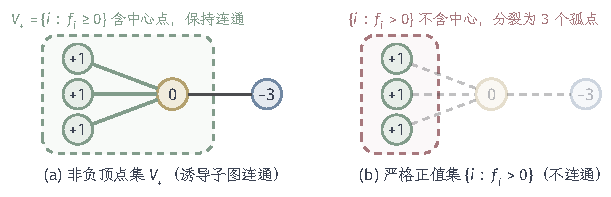
\includegraphics[width=103.396mm]{figures/03-graphs/05-matrices-and-spectra/tikz/fiedler-star-zero-center/figure.pdf}
  \caption{五顶点星图$K_{1,4}$上Fiedler向量$\bm f=(1,1,1,0,-3)^\top$的节域结构。(a) 非负集合$V_+=\{i:f_i\geq 0\}$包含取值为$0$的中心顶点，诱导子图保持连通；(b) 严格正值集合$\{i:f_i>0\}$不含中心顶点，分裂为三个孤立叶子。}
  \label{fig:graph-fiedler-star-zero}
\end{BookInlineFigure}

Fiedler向量$\bm v_2$通过一维连续坐标为所有顶点排出了反映瓶颈结构的自然顺序。在此基础上，接下来两节将进一步解决两个关键问题：第~\ref{sec:graph-cheeger}节引入归一化拉普拉斯与Cheeger不等式，严格证明沿谱方向扫描阈值必定能找到逼近全局最优导通率的稀疏割；第~\ref{sec:graph-ratiocut}至\ref{sec:graph-spectral-partition-comparison}节则给出RatioCut与NCut的完整谱划分算法。

\section{Cheeger不等式}
\label{sec:graph-cheeger}

前一节用组合拉普拉斯的第二小特征值$\lambda_2$衡量图连得有多紧。但$\lambda_2$会随边权的整体放大而增大，两张规模不同的图之间直接比较$\lambda_2$并不公平。

一种更合理的衡量方式是：割掉一组边后，组间断开的边权占较小一侧总连接量的多少？如果一座大桥连接两个城市群，桥虽然只有一条，但两侧各自有大量内部道路，切断这一条边对较小一侧的影响取决于那一侧总共有多少路。相比之下，切下一个只有一条边的孤立叶子，割权同为一，但那个叶子的全部连接就是这一条边。

以下假定正权支撑连通，这保证每个顶点都有正度。

\subsection{导通率}
\label{sec:graph-conductance}

用$S$和$\bar S=V\setminus S$表示一组顶点和剩下的顶点，要求两组都非空。把一端在$S$、另一端在$\bar S$的边各数一次，将它们的权重相加，得到\term{割权}（cut weight）$c(S,\bar S)$。

顶点$i$的加权度$d_i$是连到该点的所有边权之和。将$S$内每个点的度累加，得到集合体积$\operatorname{vol}(S)=\sum_{i\in S}d_i$。体积的计算中，组内边在两个端点各被计入一次，跨边只在组内的那个端点计入。图~\ref{fig:graph-conductance-volume}标出了这两种计数。

\begin{BookInlineFigure}
  \centering
  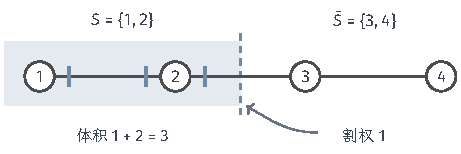
\includegraphics{figures/03-graphs/05-matrices-and-spectra/tikz/conductance-volume/figure.pdf}
  \caption{单位权四点路径上$S=\{1,2\}$的体积计算。每道刻度表示一个边端点处计入的一份。边$12$两端都在$S$中，计两份；边$23$只有一端在$S$中，计一份。左侧体积为$3$。虚线切过的边只有$23$，割权为$1$。}
  \label{fig:graph-conductance-volume}
\end{BookInlineFigure}

用体积较小的一侧来衡量规模。分母越小，同样的割权所占的比例就越大。

\begin{definition}[导通率]
\label{def:graph-conductance}
集合的\term{导通率}（conductance）和图的最小导通率分别为
\begin{equation}
\label{eq:graph-conductance}
\phi(S)=\frac{c(S,\bar S)}
  {\min\{\operatorname{vol}(S),\operatorname{vol}(\bar S)\}},
\qquad
\phi_*=\min_{\varnothing\ne S\subsetneq V}\phi(S).
\end{equation}
\end{definition}

在单位权四点路径上试两种切法。把中间边$23$切断，得到$\{1,2\}$和$\{3,4\}$。顶点$1$的度为$1$，顶点$2$的度为$2$，左侧体积为$1+2=3$。右侧的度分别为$2,1$，体积也为$3$。跨边只有一条，割权为$1$，所以这个割的导通率为$1/3$。

如果只切下端点$1$，割权仍为$1$，但$\{1\}$的体积只有$1$，另一侧体积为$5$。导通率变成$1/1=1$。

两种割的割权相同，但中间割的较小一侧承载了更多连接（体积$3$对$1$），所以按比例算，中间割更"高效"。在所有切法中选最小的导通率，就是图的$\phi_*$。

接下来要用归一化拉普拉斯的第二小特征值$\mu_2$来控制$\phi_*$。回顾第~\ref{sec:graph-normalized-laplacian}节，对称归一化拉普拉斯$\mathcal L=\bm D^{-1/2}\bm L\bm D^{-1/2}$的变分刻画为
\begin{equation}
\label{eq:graph-normalized-variational-cut}
\mu_2=\min_{\substack{\bm f^\top\bm D\bm1=0\\\bm f\ne\bm0}}
       \frac{\bm f^\top\bm L\bm f}{\bm f^\top\bm D\bm f}.
\end{equation}
这里的分母把每个坐标的平方乘以该点的度再求和，而不是简单的平方和。零方向对应的条件也变成度加权的零和$\sum_i d_i f_i=0$。若将$S$内的坐标设为$1$，其余设为$0$，分母恰好是$\operatorname{vol}(S)$。因此体积与归一化谱之间有了直接联系。

\begin{theorem}[\term{Cheeger不等式}]
\label{thm:graph-cheeger}
有限无向非负权图的正权支撑连通，且至少有两个顶点时，
\begin{equation}
\label{eq:graph-cheeger}
\frac{\mu_2}{2}\leq\phi_*\leq \sqrt{2\mu_2}.
\end{equation}
\end{theorem}

两个界各回答一个问题。下界说：无论怎样选择分组，其导通率都至少为$\mu_2/2$，图中不存在比这更稀疏的平衡割。上界则提供了一种构造性的搜索：按第二特征方向的分量给顶点排序，依次尝试切点，其中至少有一个割的导通率不超过$\sqrt{2\mu_2}$。

下面分别证明这两个界。

\subsection{下界：指示向量的Rayleigh商}
\label{sec:graph-cheeger-lower}

为证明下界，我们从任意一个割出发，构造一个满足约束的试探向量，再把它代入式~\eqref{eq:graph-normalized-variational-cut}。

取任意非空真子集$S$，设$a=\operatorname{vol}(S)\leq\operatorname{vol}(\bar S)=b$。从$S$的指示向量$\bm 1_S$出发，把每个坐标减去度加权平均值$a/(a+b)$，得到
\[
\bm f=\bm1_S-\frac{a}{a+b}\bm1.
\]
$\bm f$在$S$上取值$b/(a+b)$，在$\bar S$上取值$-a/(a+b)$。度加权的坐标和为
\[
a\cdot\frac{b}{a+b}+b\cdot\frac{-a}{a+b}=0,
\]
满足零和条件$\bm f^\top\bm D\bm 1=0$。

下面分别计算分子和分母。对组内的一条边，两端取同一个值，差为零，不贡献能量。对跨边，两端分别取$b/(a+b)$和$-a/(a+b)$，差恰好为$1$。因此分子等于割权：
\[
\bm f^\top\bm L\bm f=c(S,\bar S).
\]

分母将两侧的常数平方各按体积累加：
\[
\bm f^\top\bm D\bm f
=a\left(\frac{b}{a+b}\right)^{\!2}
+b\left(\frac{a}{a+b}\right)^{\!2}
=\frac{ab}{a+b}.
\]

$\mu_2$是所有合格向量中Rayleigh商的最小值。把$\bm f$代入，给出上界
\[
\mu_2
\leq\frac{c(S,\bar S)}{\dfrac{ab}{a+b}}
=c(S,\bar S)\left(\frac{1}{a}+\frac{1}{b}\right).
\]
因为$a\leq b$，有$1/b\leq 1/a$，所以
\[
\frac{1}{a}+\frac{1}{b}\leq\frac{2}{a}
=\frac{2}{\min\{\operatorname{vol}(S),\operatorname{vol}(\bar S)\}}.
\]
代入得$\mu_2\leq 2\phi(S)$。这个结论对每个非空真子集$S$都成立，因此对所有割取最小后，$\mu_2/2\leq\phi_*$。

用四点路径的中间割核对。两侧体积$a=b=3$，中心化后两侧的坐标分别为$1/2$和$-1/2$。只有一条跨边，割权为$1$。分母为$3\cdot(1/2)^2+3\cdot(1/2)^2=3/2$。代入得$\mu_2\leq 1/(3/2)=2/3$，恰好是$2\phi(S)=2\cdot(1/3)$。

\subsection{上界：扫描阈值}
\label{sec:graph-cheeger-sweep}

下界告诉我们导通率不可能太小。上界则要找到一个具体的割来展示它也不会太大。思路是从归一化拉普拉斯的第二特征方向出发，对顶点排序后逐个阈值切开，证明其中至少有一个割的导通率不超过$\sqrt{2\mu_2}$。

证明分三步。第一步从特征方向中选出一侧体积不超过半图的非负向量。第二步用积分论证，说明沿该向量的阈值扫描中，导通率的加权平均可以用能量商控制。第三步用Cauchy--Schwarz不等式把能量商和$\mu_2$联系起来。

\paragraph{第一步：选出合适的一侧}

设$\bm f$是式~\eqref{eq:graph-normalized-variational-cut}的一个最优向量，能量商恰为$\mu_2$。按分量从小到大排列各顶点，逐个累计加权度。累计首次达到$\operatorname{vol}(V)/2$时，取该顶点的分量值作为度加权中位数$\tau$。严格小于$\tau$的顶点体积不超过半图，严格大于$\tau$的也不超过半图。

将$\bm f$平移为$\bm h=\bm f-\tau\bm 1$。平移对每条边的差没有影响，所以能量$\bm h^\top\bm L\bm h=\bm f^\top\bm L\bm f$不变。对于度加权平方和，展开得到
\[
\bm h^\top\bm D\bm h
=\bm f^\top\bm D\bm f
-2\tau\underbrace{\bm f^\top\bm D\bm 1}_{=\,0}
+\tau^2\operatorname{vol}(V)
=\bm f^\top\bm D\bm f+\tau^2\operatorname{vol}(V).
\]
分子不变，分母没有减小，因此$\bm h$的能量商不超过$\mu_2$。

把$\bm h$分成正部$\bm g^+$和负部$\bm g^-$两个非负向量：$g^+_i=\max(h_i,0)$，$g^-_i=\max(-h_i,0)$。它们的度加权平方和相加恰等于$\bm h$的度加权平方和。

逐边比较能量。若两端同号（均正或均负），差完全保留在同一部分中。若一端为$p>0$、另一端为$-q<0$，原来的差平方为$(p+q)^2$，而拆开后正部贡献$p^2$，负部贡献$q^2$，合计$p^2+q^2\leq(p+q)^2$。因此两部分的能量之和不超过原来的能量。

如果两个非零部分的能量商都严格大于$\mu_2$，把它们的能量分别用$\mu_2$乘平方和的下界代入，加起来就会超过$\mu_2$乘原平方和，而左侧能量之和又不超过原能量——矛盾。所以至少有一个非零部分$\bm g$的能量商不超过$\mu_2$。这个$\bm g$非负，且它的非零支撑的体积至多为$\operatorname{vol}(V)/2$。

\paragraph{第二步：积分论证}

对$t\geq0$，定义集合$S_t=\{i:g_i^2>t\}$。随着$t$增大，$S_t$逐渐缩小。$t$的连续变化只在经过某个$g_i^2$时才改变集合，因此实际上只需处理有限个阈值。

先计算体积对阈值的积分。顶点$i$当且仅当$0\leq t<g_i^2$时被$S_t$选入，此时它对体积的贡献为$d_i$。把所有顶点的贡献积起来，
\[
\int_0^\infty\operatorname{vol}(S_t)\,\mathrm dt
=\sum_i d_ig_i^2.
\]

再计算割权的积分。对一条边$\{i,j\}$，不妨设$g_i\geq g_j\geq 0$。当$g_j^2\leq t<g_i^2$时，$i$入选但$j$未入选，这条边被切过，贡献$w_{i,j}$。因此
\[
\int_0^\infty c(S_t,\bar S_t)\,\mathrm dt
=\sum_{\{i,j\}\in E}w_{i,j}|g_i^2-g_j^2|.
\]

每个非空$S_t$都在$\bm g$的非零支撑中，体积不超过$\operatorname{vol}(V)/2$。在任一非空的常值区间内，割权等于该割的导通率乘以该集合的体积（因为$\operatorname{vol}(S_t)$已经是较小一侧）。因此两个积分的比值是各割导通率按"区间长度乘体积"为权的加权平均。加权平均不会小于所有项的最小值，所以至少有一个阈值$t_0$使得
\[
\phi(S_{t_0})
\leq\frac{\displaystyle\sum_{\{i,j\}}w_{i,j}|g_i^2-g_j^2|}
         {\displaystyle\sum_i d_ig_i^2}.
\]

\paragraph{第三步：Cauchy--Schwarz}

因为$\bm g$非负，可以把$|g_i^2-g_j^2|$因式分解为$|g_i-g_j|\cdot(g_i+g_j)$。对以边为下标的两个向量——一个分量为$\sqrt{w_{i,j}}|g_i-g_j|$，另一个为$\sqrt{w_{i,j}}(g_i+g_j)$——应用Cauchy--Schwarz不等式：
\[
\sum_{\{i,j\}}w_{i,j}|g_i^2-g_j^2|
\leq
\sqrt{\sum_{\{i,j\}}w_{i,j}(g_i-g_j)^2}
\cdot
\sqrt{\sum_{\{i,j\}}w_{i,j}(g_i+g_j)^2}.
\]
第一个因子的平方正是沿边能量$\bm g^\top\bm L\bm g$。对第二个因子，用$(g_i+g_j)^2\leq 2(g_i^2+g_j^2)$放大，然后逐个顶点$i$收集所有与它相接的边权，得到$d_i$倍的$g_i^2$，因此
\[
\sum_{\{i,j\}}w_{i,j}(g_i+g_j)^2
\leq 2\sum_i d_ig_i^2.
\]

把两个因子代入第二步的比值，再除以分母$\sum_i d_ig_i^2$，得到
\[
\phi(S_{t_0})
\leq\frac{\sqrt{\bm g^\top\bm L\bm g}\cdot\sqrt{2\sum_i d_ig_i^2}}
         {\sum_i d_ig_i^2}
=\sqrt{\frac{2\,\bm g^\top\bm L\bm g}{\bm g^\top\bm D\bm g}}.
\]
由$\bm g$的能量商不超过$\mu_2$，得到$\phi(S_{t_0})\leq\sqrt{2\mu_2}$。

\paragraph{从$\bm g$的阈值回到$\bm f$的排序}

实际操作时，不需要先平移、再取正负部。如果$\bm g$来自正部（即$\bm h$的正值一侧），它的非零支撑恰好是$\bm f$中值较大的那些顶点。如果来自负部，则对应$\bm f$中值较小的那些。因此可以直接对$\bm f$排序，扫描从最大端或最小端开始的前缀。尾端的割与其补集给出同一个分组，所以相同坐标的顶点必须整组跨过阈值，不能任意拆开。

\begin{figure}[htbp]
\centering
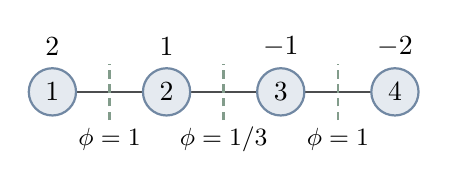
\begin{tikzpicture}[
  x=1.45cm,y=1cm,
  vertex/.style={circle,draw=graphSweepBlue,fill=graphSweepLight,
    line width=.8pt,minimum size=6mm,inner sep=0pt},
  cut/.style={draw=graphSweepGreen,densely dashed,line width=.85pt}
]
\definecolor{graphSweepBlue}{HTML}{7188A3}
\definecolor{graphSweepLight}{HTML}{E5EAF0}
\definecolor{graphSweepGreen}{HTML}{829C8B}
\definecolor{graphSweepLine}{HTML}{4C4D4F}
\draw[graphSweepLine,line width=.85pt] (0,0)--(3,0);
\foreach \i/\v/\f in {0/1/2,1/2/1,2/3/-1,3/4/-2}{
   \node[vertex] at (\i,0) {$\v$};
   \node at (\i,.57) {$\f$};
}
\foreach \i/\value in {.5/1,1.5/{1/3},2.5/1}{
   \draw[cut] (\i,-.36)--(\i,.35);
   \node[font=\small] at (\i,-.6) {$\phi=\value$};
}
\end{tikzpicture}

\caption{单位权四顶点路径上的阈值扫描。顶点上方标出了归一化谱方向还原后的函数值。三条竖虚线对应三个候选阈值，每个阈值恰好切过一条边。}
\label{fig:graph-cheeger-path-sweep}
\end{figure}

用四点路径验证。各点度为$(1,2,2,1)$。取$\bm f=(2,1,-1,-2)^\top$，计算
\[
\bm L\bm f=(1,1,-1,-1)^\top=\tfrac12\bm D\bm f,
\]
可知$\bm f$确实是归一化特征值$\mu_2=1/2$对应的方向。负值侧和正值侧的体积各为$3$，取中位数$\tau=0$后正部为$\bm g=(2,1,0,0)^\top$。

沿边能量为$(2-1)^2+(1-0)^2+(0-0)^2=2$，度加权平方和为$1\cdot4+2\cdot1=6$，能量商为$2/6=1/3<\mu_2$。

$g_i^2$的取值为$(4,1,0,0)$，产生两个非空阈值区间。图~\ref{fig:graph-cheeger-threshold-intervals}在同一条阈值轴上标出了顶点入选和边被切过的区间。

\begin{BookInlineFigure}
  \centering
  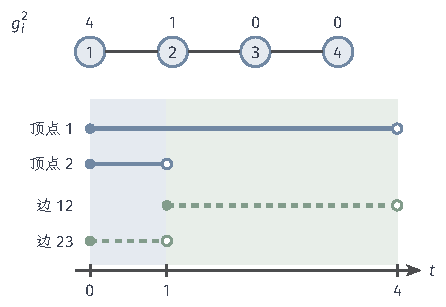
\includegraphics{figures/03-graphs/05-matrices-and-spectra/tikz/cheeger-threshold-intervals/figure.pdf}
  \caption{对$g_i^2=(4,1,0,0)_i$扫描阈值$t$。实线段标出顶点入选的区间，虚线段标出边跨割的区间。顶点$3,4$始终不入选，边$34$始终不被切过。}
  \label{fig:graph-cheeger-threshold-intervals}
\end{BookInlineFigure}

区间$[0,1)$选入$\{1,2\}$，体积$3$，割权$1$（边$23$被切），导通率$1/3$。区间$[1,4)$只选入$\{1\}$，体积$1$，割权$1$（边$12$被切），导通率$1$。

体积积分为$1\cdot3+3\cdot1=6$，割权积分为$1\cdot1+3\cdot1=4$。比值$4/6=2/3$，恰好位于两个导通率$1/3$和$1$之间。上界要求至少有一个候选不超过$\sqrt{2\cdot1/2}=1$，中间割的$1/3$远远满足。

直接按$\bm f$排序时，还有一个候选是$\{1,2,3\}$，它也只切过一条边，导通率为$1/3$。三个候选都只切一条边，中间位置的小侧体积最大，导通率最低。

\subsection{两端的紧性}
\label{sec:graph-cheeger-tightness}

Cheeger不等式的两端不能同时改进为同一个线性关系。下面通过两族图分别说明下界和上界各自的紧性。

\paragraph{下界取等：超立方体}

$d$维超立方体的$2^d$个顶点各有$d$条边，是$d$正则图。组合拉普拉斯的第二小特征值为$2$（沿任一坐标交替赋值$\pm1$给出这个值）。归一化后$\mu_2=2/d$。

沿某一坐标把顶点等分为两半。每个顶点恰有一条边跨割，每侧体积为$2^{d-1}\cdot d$。导通率为$2^{d-1}/(2^{d-1}\cdot d)=1/d$，恰好等于$\mu_2/2$。结合下界$\phi_*\geq\mu_2/2=1/d$，可以断定$\phi_*=1/d$。这说明下界的等号确实可以达到。

\paragraph{上界中的平方根尺度：长环}

对偶数$n\geq4$的环$C_n$，每个非平凡割至少切过两条边。取相邻的$n/2$个顶点为一侧，割权为$2$，该侧体积为$n/2\cdot 2=n$，导通率为$2/n$。可以验证这就是最小导通率$\phi_*=2/n$。

归一化拉普拉斯的第二小特征值为
\[
\mu_2=1-\cos(2\pi/n).
\]
当$n$增大时，$1-\cos(2\pi/n)\approx 2\pi^2/n^2$，因此$\mu_2$是$n^{-2}$阶的量，而$\phi_*=2/n$是$n^{-1}$阶的量。两者之间确实存在平方根的尺度差距：$\phi_*$与$\sqrt{\mu_2}$同阶。这说明上界$\phi_*\leq\sqrt{2\mu_2}$中的平方根不是证明技巧造成的损失，而是反映了长环这类图的真实结构。

这两族图放在一起看，下界可以精确取等，上界中的平方根指数不能改进。但两端并不在同一族图上同时取等——超立方体实现了下界的常数，长环展示了上界的指数。

\section{RatioCut谱划分}
\label{sec:graph-ratiocut}

给定一张图，要把顶点分成两个非空组。边的两个端点分在不同组时，需要付出这条边的权重。如果只求割权最小，把一个度最低的顶点单独切出来往往就够了，但这样的分组并不平衡。\term{RatioCut}用两侧的顶点数量调整割权，使得切出很小一组的方案被放大惩罚。

\subsection{RatioCut的谱松弛}
\label{sec:graph-ratiocut-relaxation}

设第一组为$S$，第二组为$\bar S=V\setminus S$，两组的顶点数分别为$s=|S|$和$t=|\bar S|$，满足$s+t=n$。将割权分别除以两组大小，再相加，定义
\begin{equation}
\label{eq:graph-ratiocut}
\operatorname{RatioCut}(S)=c(S,\bar S)\left(\frac{1}{s}+\frac{1}{t}\right).
\end{equation}
若两种切法的割权相同，其中一种只留下很小的一组，那个组对应的倒数$1/s$就会很大，整体代价随之增大。

在四点路径上，切下端点$1$得到一对三的分组，割权为$1$，代价为$1\cdot(1+1/3)=4/3$。切断中间边得到二对二的分组，割权也为$1$，代价为$1\cdot(1/2+1/2)=1$。中间割在RatioCut意义下更优。

目标是在所有非空二分中找出代价最小的分组。为了用拉普拉斯的谱工具求解，我们先把分组编码为一个向量。

给$S$上的顶点赋$1$，$\bar S$上的赋$0$，得到指示向量$\bm 1_S$。跨边的两端相差$1$，组内边的两端相差$0$，因此沿边能量$\bm 1_S^\top\bm L\bm 1_S$恰好等于割权$c(S,\bar S)$。

但这个向量的坐标和为$s$，不满足式~\eqref{eq:graph-algebraic-connectivity}的正交条件$\bm x\perp\bm 1$。将每个坐标减去均值$s/n$，得到
\[
\bm y=\bm 1_S-\frac{s}{n}\bm 1.
\]
$\bm y$在$S$上取$t/n$，在$\bar S$上取$-s/n$。两侧之差仍为$t/n-(-s/n)=1$，跨边的能量不变，组内边仍无贡献。因此$\bm y^\top\bm L\bm y=c(S,\bar S)$。

向量的长度平方按两侧计算：
\[
\bm y^\top\bm y
=s\left(\frac{t}{n}\right)^{\!2}+t\left(\frac{s}{n}\right)^{\!2}
=\frac{st}{n}.
\]
将$\bm y$归一化为$\bm x=\bm y/\|\bm y\|$，它的长度变为$1$，坐标和仍为$0$。能量被除以$\|\bm y\|^2=st/n$，得到
\[
\bm x^\top\bm L\bm x
=\frac{n}{st}\,c(S,\bar S)
=c(S,\bar S)\left(\frac{1}{s}+\frac{1}{t}\right)
=\operatorname{RatioCut}(S).
\]
最后一步用到$n/(st)=1/s+1/t$。这就解释了两组顶点数的倒数之和为什么会出现。

以四点路径的中间割为例，$s=t=2$，归一化后的向量为$(1/2,1/2,-1/2,-1/2)^\top$。唯一的非零边差等于$1$，能量为$1$，恰好等于这个割的RatioCut值。

到此为止，向量$\bm x$只能取由分组确定的两个值。这个离散限制使得问题在组合意义上是困难的。谱松弛去掉两值限制，只保留$\bm x\perp\bm 1$和$\|\bm x\|=1$这两个条件。松弛后的最小值就是组合拉普拉斯的第二小特征值$\lambda_2$。

原来的每个分组向量都满足这两个条件，因而$\lambda_2$不超过任何实际RatioCut值。它是离散最优值的一个下界。

图~\ref{fig:graph-ratiocut-relaxation}对比了实际分组和松弛解。中间割的两值向量只在一条边上有变化，所有能量集中在那里。松弛解允许数值在多条边上逐步过渡，沿边能量因此更小。

\begin{BookInlineFigure}
  \centering
  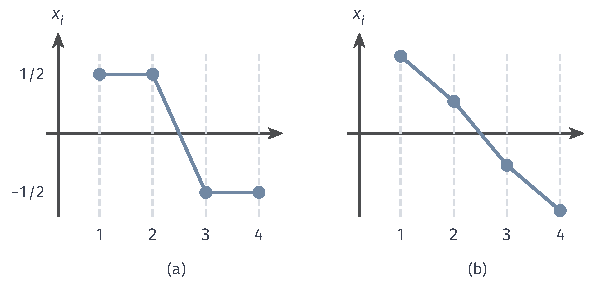
\includegraphics{figures/03-graphs/05-matrices-and-spectra/tikz/ratiocut-relaxation/figure.pdf}
  \caption{单位权四点路径的两种赋值。横轴按路径顺序标出顶点，纵轴是赋值。(a) 中间割的两值向量，能量为$1$。(b) 松弛后得到的第二特征向量，能量为$2-\sqrt2$。两者的坐标和都为零，长度都为一。}
  \label{fig:graph-ratiocut-relaxation}
\end{BookInlineFigure}

松弛给出了下界和一个连续方向，但这个方向本身不是合法的分组。下一步要把实数值的特征向量转换成可以在原图中使用的两组顶点。

\subsection{算法实现}
\label{sec:graph-ratiocut-sweep}

思路是按特征向量的分量从大到小排序，在相邻不同值之间逐个试切，并为每个候选分组计算原始的RatioCut目标。

\begin{algorithm}[RatioCut阈值扫描]
\label{alg:graph-ratiocut-sweep}
给定有限非负加权图，输出非空二分及其RatioCut值。
\begin{enumerate}
\item 若图不连通，选一个连通分量为一侧，另一侧为其余顶点。两侧之间没有正权边，割权为零，返回零代价的分组。
\item 否则求组合拉普拉斯的第二特征向量。按分量从大到小排序。分量相同的顶点作为一组，不能拆开。
\item 从空集开始逐组加入顶点。加入时更新割权：从当前割权中减去新顶点连向已选顶点的边权（这些边从跨边变为组内边），加上连向仍未入选顶点的边权（这些边从组内边变为跨边）。
\item 每组加入后，若两侧均非空，按式~\eqref{eq:graph-ratiocut}计算RatioCut。比较所有候选，返回目标值最小的分组。
\end{enumerate}
\end{algorithm}

\paragraph{执行过程}

在单位权四点路径上，第二特征向量可取为
\[
\bm x=(a,b,-b,-a)^\top,
\qquad a=\cos(\pi/8),\quad b=\cos(3\pi/8).
\]
因为$a>b>0$，顶点按$1,2,3,4$的顺序入选。

第一步放入顶点$1$。它只有一条边连向尚未入选的顶点$2$，割权变为$1$。第二步放入$2$时，边$12$从跨边变成组内边（割权减$1$），但边$23$从组内变为跨边（割权加$1$），割权仍为$1$。第三步放入$3$时，类似地跨边改成$34$。

三个候选的计算如下。
\begin{center}
\begin{tabular}{lccc}
\toprule
已选集合 & 两侧大小 & 割权 & RatioCut\\
\midrule
$\{1\}$ & $1,3$ & $1$ & $4/3$\\
$\{1,2\}$ & $2,2$ & $1$ & $1$\\
$\{1,2,3\}$ & $3,1$ & $1$ & $4/3$\\
\bottomrule
\end{tabular}
\end{center}

图~\ref{fig:ratiocut-sweep-candidates}按排序顺序画出四个顶点，并标出三种切分位置。每条竖线对应一种候选，线两侧的集合、割边及RatioCut值都标在旁边。观察中间切法如何同时使两侧大小均匀且割权不增。

\begin{figure}[!htb]
\centering
\begin{tikzpicture}[x=1mm,y=1mm,>=Stealth,
  vertex/.style={circle,draw=FigureBlue,fill=FigureBlueFill,inner sep=0pt,
    minimum size=5mm,line width=.52pt,font=\figurefont\fontsize{8}{10}\selectfont},
  cutline/.style={dashed,FigureRed,line width=.6pt},
  clabel/.style={font=\figurefont\fontsize{7}{8.5}\selectfont,FigureRed},
  vlabel/.style={font=\figurefont\fontsize{7.5}{9}\selectfont,FigureInk}]
  % vertices on a line
  \node[vertex] (v1) at (0,0) {$1$};
  \node[vertex] (v2) at (16,0) {$2$};
  \node[vertex] (v3) at (32,0) {$3$};
  \node[vertex] (v4) at (48,0) {$4$};
  \draw[FigureStroke,line width=.52pt] (v1)--(v2)--(v3)--(v4);
  % Cut 1: after vertex 1
  \draw[cutline] (8,7) -- (8,-7);
  \node[clabel,above] at (8,7.5) {$\frac{4}{3}$};
  % Cut 2: after vertex 2
  \draw[cutline] (24,7) -- (24,-7);
  \node[clabel,above] at (24,7.5) {$1$};
  % Cut 3: after vertex 3
  \draw[cutline] (40,7) -- (40,-7);
  \node[clabel,above] at (40,7.5) {$\frac{4}{3}$};
  % vertex ordering label
  \node[vlabel] at (24,-12) {按特征向量分量从大到小排序};
\end{tikzpicture}
\caption{四点路径上的RatioCut阈值扫描。四个顶点按第二特征向量分量递减排列。红色虚线标出三种切分位置，上方数字是对应的RatioCut值。中间割的代价最低。}
\label{fig:ratiocut-sweep-candidates}
\end{figure}

中间割的代价最小，为$1$。这是扫描得到的实际分组代价，可以和松弛下界$\lambda_2=2-\sqrt2\approx0.586$放在一起比较。

\subsection{算法分析}
\label{sec:graph-ratiocut-guarantee}

记所有非空二分中的RatioCut最小值为$\operatorname{OPT}_R$，扫描返回的分组为$S_R$。松弛扩大了可行域，给出下界；扫描提供了一个具体的可行割，给出上界：
\begin{equation}
\label{eq:graph-ratiocut-bounds}
\lambda_2\leq\operatorname{OPT}_R
\leq\operatorname{RatioCut}(S_R).
\end{equation}

四点路径上可以直接验证$\operatorname{OPT}_R=1$。任何非空二分至少切过一条边（路径是连通的），且两侧顶点数之积$st$至多为$\lfloor n/2\rfloor\cdot\lceil n/2\rceil=4$。因此$1/s+1/t=n/(st)\geq 4/4=1$，任何割的RatioCut都不低于$1$。中间割恰好达到了这个值。

排序$n$个顶点需要$O(n\log n)$时间。扫描过程中每个顶点加入一次，加入时检查它的邻接表，因此所有边在两个端点各被访问至多一次，扫描耗时$O(n+m)$。求特征向量的代价另行计算，取决于所用的迭代方法和精度要求。

一次扫描只比较沿一个排序方向切开的嵌套集合，没有覆盖全部$2^{n-1}-1$个无序二分。选择不同的最优方向（当$\lambda_2$为重根时）或近似方向可能给出不同的候选。相同分量作为一组处理，减少了切点数量。

精确的$\lambda_2$是有效的下界。但如果使用的是数值迭代得到的近似特征向量，代入Rayleigh商所得的值大于或等于$\lambda_2$，不一定仍是离散最优值的下界。报告结果时应区分：认证过误差的下界和数值估计值。扫描得到的分组及其原目标代价可以直接在原图上核对，不受特征向量精度的影响。

\section{NCut谱划分}
\label{sec:graph-ncut}

RatioCut在割权相同时偏好顶点数较均衡的划分，但顶点数不反映每个顶点参与连接的多少。例如，把星图的多个叶子归为一组，这组顶点内部没有边，其全部度数都来自跨组连接。若希望比较每侧跨组连接占该侧总连接量的比例，可以把分母换成集合体积。体积包括内部边和跨割边的贡献，不能直接等同于内部边权或内部连接密度。

为此，Shi与Malik于2000年提出将RatioCut分母中的“节点个数$|A|,|B|$”替换为子图中所有节点的\emph{度数之和}（即第~\ref{sec:graph-conductance}小节定义的集合体积$\operatorname{vol}(A),\operatorname{vol}(B)$），从而得到了\term{归一化割}（normalized cut，简称\term{NCut}）\scite{shi2000normalized}。

以下先限制在正度顶点集$V_+$上，并假定$V_+$非空；无自环图中这保证$|V_+|\geq2$。若全图没有正权边，则不存在两侧均为正体积的合法NCut划分。

\subsection{NCut的谱松弛}
\label{sec:graph-ncut-relaxation}

\begin{definition}[NCut目标]
\label{def:graph-ncut}
设非空二分$(A,B)$（其中$B=V\setminus A$）两侧的体积分别为$\operatorname{vol}(A)=\sum_{i\in A}d_i>0$和$\operatorname{vol}(B)=\sum_{j\in B}d_j>0$（满足$\operatorname{vol}(A)+\operatorname{vol}(B)=\operatorname{vol}(V)$）。划分$(A,B)$的归一化割（NCut）目标定义为
\begin{equation}
\label{eq:graph-ncut}
\operatorname{NCut}(A,B)
=\frac{c(A,B)}{\operatorname{vol}(A)}+\frac{c(A,B)}{\operatorname{vol}(B)}
=c(A,B)\left(\frac{1}{\operatorname{vol}(A)}+\frac{1}{\operatorname{vol}(B)}\right).
\end{equation}
\end{definition}

由$\operatorname{vol}(A)=2w(E(A))+c(A,B)$可得，当$c(A,B)/\operatorname{vol}(A)$较小时，$A$的度数总和主要来自内部边；另一侧同理。因此，NCut较小表示两侧各自只有较小比例的连接权重通向外部，并不保证内部连通或内部边密度较高。全图体积固定时，体积平衡也是目标的一部分，但不能同时独立最大化两侧体积。

\begin{BookInlineFigure}
  \centering
  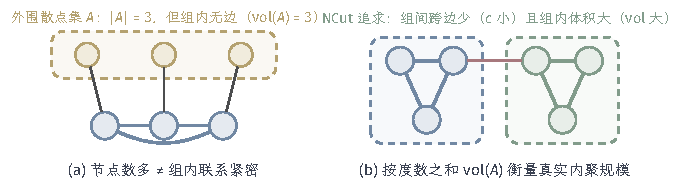
\includegraphics[width=114.935mm]{figures/03-graphs/05-matrices-and-spectra/tikz/ncut-volume-vs-count/figure.pdf}
  \caption{为什么NCut用度数总和（体积$\operatorname{vol}(A)$）替代节点个数$|A|$。(a) 将$3$个外围叶子归为集合$A$时，虽然节点数$|A|=3$已占半图，但$A$内部没有一条边，体积仅为$\operatorname{vol}(A)=3$。(b) 将两个内部紧密相连的三角形社区切开时，仅断开$1$条红边，而两侧体积各达$\operatorname{vol}=7$，两侧的跨割权与体积之比均为$1/7$。}
  \label{fig:graph-ncut-volume-vs-count}
\end{BookInlineFigure}

与第~\ref{sec:graph-ratiocut-relaxation}小节的RatioCut推导完全平行，只需把顶点个数$|A|,|B|$替换为集合体积$\operatorname{vol}(A),\operatorname{vol}(B)$，并把标准欧氏内积替换为以度矩阵$\bm D$加权的内积，即可分四步导出NCut的谱松弛。

\paragraph{1. 构造按体积加权的指示向量$\bm f$}

对任意满足$\operatorname{vol}(A)>0,\operatorname{vol}(B)>0$的二分$(A,B)$，利用两侧体积的比值构造两值指示向量$\bm f=(f_1,\ldots,f_n)^\top\in\mathbb R^n$：
\begin{equation}
\label{eq:ncut-indicator-vector}
  f_i = \begin{cases}
    \sqrt{\dfrac{\operatorname{vol}(B)}{\operatorname{vol}(A)}}, & i\in A,\\[10pt]
    -\sqrt{\dfrac{\operatorname{vol}(A)}{\operatorname{vol}(B)}}, & i\in B.
  \end{cases}
\end{equation}

\paragraph{2. 代入二次型分子$\bm f^\top\bm L\bm f$}

将$\bm f$代入组合拉普拉斯二次型$\bm f^\top\bm L\bm f=\sum_{\{i,j\}\in E}w_{i,j}(f_i-f_j)^2$。组内边两端取值相同、差为$0$；每条跨割边两端取值差的平方为
\[
\begin{aligned}
  \left(\sqrt{\frac{\operatorname{vol}(B)}{\operatorname{vol}(A)}} - \left(-\sqrt{\frac{\operatorname{vol}(A)}{\operatorname{vol}(B)}}\right)\right)^{\!2}
  &= \frac{\operatorname{vol}(B)}{\operatorname{vol}(A)} + \frac{\operatorname{vol}(A)}{\operatorname{vol}(B)} + 2 \\
  &= \operatorname{vol}(V)\left(\frac{1}{\operatorname{vol}(A)}+\frac{1}{\operatorname{vol}(B)}\right).
\end{aligned}
\]
对所有跨割边加权求和，得到二次型分子：
\begin{equation}
\label{eq:ncut-quadratic-numerator}
  \bm f^\top\bm L\bm f = \operatorname{vol}(V)\,c(A,B)\left(\frac{1}{\operatorname{vol}(A)}+\frac{1}{\operatorname{vol}(B)}\right)
  = \operatorname{vol}(V)\,\operatorname{NCut}(A,B).
\end{equation}

\paragraph{3. 验证度加权分母和度加权正交条件}

由于式~\eqref{eq:ncut-indicator-vector}使用的是体积比值，对应的正交条件和范数分母也自然带有顶点度数$d_i$的权重（即度对角矩阵$\bm D$）。第一，计算度加权坐标和$\bm f^\top\bm D\bm 1$：
\[
\begin{aligned}
  \bm f^\top\bm D\bm 1
  = \sum_{i=1}^n d_i f_i
  &= \left(\sum_{i\in A}d_i\right)\sqrt{\frac{\operatorname{vol}(B)}{\operatorname{vol}(A)}}
    - \left(\sum_{j\in B}d_j\right)\sqrt{\frac{\operatorname{vol}(A)}{\operatorname{vol}(B)}} \\
  &= \sqrt{\operatorname{vol}(A)\operatorname{vol}(B)} - \sqrt{\operatorname{vol}(A)\operatorname{vol}(B)}
  = 0.
\end{aligned}
\]
即向量$\bm f$恒满足度加权零和条件$\bm D\bm 1\perp\bm f$。

第二，计算度加权长度平方（分母$\bm f^\top\bm D\bm f$）：
\[
\begin{aligned}
  \bm f^\top\bm D\bm f
  = \sum_{i=1}^n d_i f_i^2
  &= \operatorname{vol}(A)\cdot\frac{\operatorname{vol}(B)}{\operatorname{vol}(A)}
    + \operatorname{vol}(B)\cdot\frac{\operatorname{vol}(A)}{\operatorname{vol}(B)} \\
  &= \operatorname{vol}(B) + \operatorname{vol}(A)
  = \operatorname{vol}(V).
\end{aligned}
\]
将分子式~\eqref{eq:ncut-quadratic-numerator}除以分母$\bm f^\top\bm D\bm f=\operatorname{vol}(V)$，常因子$\operatorname{vol}(V)$消去，得到广义Rayleigh商恒等式：
\begin{equation}
\label{eq:ncut-rayleigh-identity}
  \operatorname{NCut}(A,B) = \frac{\bm f^\top\bm L\bm f}{\bm f^\top\bm D\bm f}.
\end{equation}

\paragraph{4. 等价变换与连续松弛}

离散NCut问题要求$f_i$取式~\eqref{eq:ncut-indicator-vector}中由划分确定的两个值。放宽这一离散限制、允许$\bm f\in\mathbb R^n$取任意满足$\bm f^\top\bm D\bm 1=0$的非零实向量，并在正度顶点空间上作可逆坐标变换$\bm z=\bm D^{1/2}\bm f$（即$\bm f=\bm D^{-1/2}\bm z$），则正交约束$\bm f^\top\bm D\bm 1=0$化为$\bm z\perp\bm D^{1/2}\bm 1$，目标函数化为对称归一化拉普拉斯$\mathcal L=\bm D^{-1/2}\bm L\bm D^{-1/2}$的标准Rayleigh商：
\begin{equation}
\label{eq:ncut-spectral-relaxation}
  \min_{\substack{\bm f^\top\bm D\bm 1=0\\\bm f\neq\bm 0}}\frac{\bm f^\top\bm L\bm f}{\bm f^\top\bm D\bm f}
  = \min_{\substack{\bm z\perp\bm D^{1/2}\bm 1\\\bm z\neq\bm 0}}\frac{\bm z^\top\mathcal L\bm z}{\bm z^\top\bm z}
  = \mu_2(\mathcal L).
\end{equation}
由此可知：NCut连续松弛问题的最小值恰为对称归一化拉普拉斯的第二小特征值$\mu_2(\mathcal L)$；若达到$\mu_2(\mathcal L)$的特征向量为$\bm z_2$，则还原到原顶点空间的连续最优解为$\bm f^\star=\bm D^{-1/2}\bm z_2$，它直接满足广义特征方程$\bm L\bm f^\star=\mu_2\bm D\bm f^\star$（即随机游走归一化拉普拉斯特征方程$\bm L_{\mathrm{rw}}\bm f^\star=\mu_2\bm f^\star$）。

\begin{theorem}[NCut的度加权二次型表示与谱松弛下界]
\label{prop:graph-ncut-relaxation}
对任意两侧体积均为正的划分$(A,B)$，按式~\eqref{eq:ncut-indicator-vector}定义的指示向量$\bm f$（或其度加权单位化向量$\bm f_A=\bm f/\sqrt{\operatorname{vol}(V)}$）满足$\bm f^\top\bm D\bm 1=0$且$\operatorname{NCut}(A,B)=\frac{\bm f^\top\bm L\bm f}{\bm f^\top\bm D\bm f}$。因而，所有合法二分的离散最优值$\operatorname{OPT}_N=\min_{\operatorname{vol}(A),\operatorname{vol}(B)>0}\operatorname{NCut}(A,B)$以正度顶点集上对称归一化拉普拉斯$\mathcal L$的第二小特征值$\mu_2$为下界：
\[
  \mu_2(\mathcal L)
  = \min_{\substack{\bm f^\top\bm D\bm 1=0\\\bm f\neq\bm 0}}\frac{\bm f^\top\bm L\bm f}{\bm f^\top\bm D\bm f}
  = \min_{\substack{\bm z\perp\bm D^{1/2}\bm 1\\\lVert\bm z\rVert_2=1}}\bm z^\top\mathcal L\bm z
  \leq \operatorname{OPT}_N.
\]
\end{theorem}

注意$\mu_2$始终在正度顶点集$V_+=\{i\in V:d_i>0\}$上计算：度数为$0$的孤立顶点既不贡献割权也不贡献体积，可在正度顶点划分完毕后归入任意一侧。

\subsection{算法实现}
\label{sec:graph-ncut-sweep}

\paragraph{主要思路与算法步骤}

NCut谱划分的整体框架与RatioCut一致，核心差别在于将矩阵从组合拉普拉斯$\bm L$换成了对称归一化拉普拉斯$\mathcal L=\bm D^{-1/2}\bm L\bm D^{-1/2}$，并且在求得$\mathcal L$的特征向量$\bm z_2$后，必须左乘$\bm D^{-1/2}$作\emph{坐标逆缩放还原}，得到原顶点空间上的谱坐标$\bm f=\bm D^{-1/2}\bm z_2$后再执行排序或聚类。

具体执行流程分为以下四步：
\begin{enumerate}
\item \emph{构建归一化拉普拉斯矩阵}：在正度顶点集上计算对称归一化拉普拉斯矩阵$\mathcal L = \bm D^{-1/2}\bm L\bm D^{-1/2} = \bm I - \bm D^{-1/2}\bm W\bm D^{-1/2}$。
\item \emph{求解归一化特征向量}：计算$\mathcal L$的第二小特征值$\mu_2$对应的特征向量$\bm z_2\in\mathbb R^n$（若作$k$路谱聚类，则求$\mathcal L$前$k$个最小特征值对应的特征向量$\bm z_1,\bm z_2,\ldots,\bm z_k$）。
\item \emph{坐标逆缩放与构建特征矩阵}：在二分问题中，将特征向量$\bm z_2$的每个分量除以对应顶点度数的平方根$\sqrt{d_i}$，还原为原顶点指示空间上的谱坐标向量$\bm f=\bm D^{-1/2}\bm z_2$（即$f_i=(\bm z_2)_i/\sqrt{d_i}$）；在$k$路谱聚类（Ng--Jordan--Weiss算法）中，将$\bm D^{-1/2}[\bm z_1,\ldots,\bm z_k]$（或直接将$[\bm z_1,\ldots,\bm z_k]$）的每一行归一化为单位长度行向量，构建特征矩阵$\bm V\in\mathbb R^{n\times k}$。
\item \emph{离散化还原（还原为最终切分）}：在二分问题中，将全部顶点按还原后的坐标$f_i$从大到小排序，依次扫描$n-1$个前缀切口，计算各自的$\operatorname{NCut}(S,\bar S)$并取最小值对应的划分输出（在$k$路划分中则对特征矩阵$\bm V$的行向量运行$k$-means聚类）。
\end{enumerate}

\begin{algorithm}[NCut谱划分]
\label{alg:graph-ncut-sweep}
给定正度支撑非空且连通的有限无向非负加权图$\mathcal G=(V,E,w)$，输出两侧为正体积的二分$(A,B)$及其NCut值。
\begin{enumerate}
\item \textbf{构建归一化矩阵}：在正度支撑上构建对称归一化拉普拉斯矩阵$\mathcal L=\bm D^{-1/2}\bm L\bm D^{-1/2}$。
\item \textbf{求解特征向量并还原坐标}：求$\mathcal L$的第二小特征值$\mu_2$对应的特征向量$\bm z_2$，作逆缩放还原$\bm f=\bm D^{-1/2}\bm z_2$（即$f_i=(\bm z_2)_i/\sqrt{d_i}$）。
\item \textbf{按还原坐标排序}：按$f_i$从大到小排列顶点，分量值相同的并列顶点整组跨过阈值。
\item \textbf{离散化还原（增量阈值扫描）}：按排序顺序逐组将顶点并入前缀集合$S$，用算法~\ref{alg:graph-ratiocut-sweep}的方式增量更新割权$c(S,\bar S)$，同时累加集合体积$\operatorname{vol}(S)=\sum_{i\in S}d_i$。对所有两侧体积均为正的候选$S$，按式~\eqref{eq:graph-ncut}计算$\operatorname{NCut}(S,\bar S)$（同时可记录导通率$\phi(S)$），返回NCut最小的划分$(A,B)$，并把原图孤点归入任意一侧。
\end{enumerate}
\end{algorithm}

\paragraph{为什么必须用还原后的$f_i$排序？}

在第二步到第三步中，有一个极易忽略的关键细节：对称矩阵特征求解器算出的是$\bm z_2$，而我们在式~\eqref{eq:ncut-indicator-vector}中构造的两值分组向量是$\bm f=\bm D^{-1/2}\bm z_2$。由于不同顶点的度数$d_i$不同，除以$\sqrt{d_i}$可能会反转两个顶点的先后顺序。

图~\ref{fig:graph-ncut-coordinate-order}用一个简单例子展示了这种顺序反转：设圆点顶点的真实谱坐标为$f_1=2$、度数为$d_1=1$；方点顶点的真实谱坐标为$f_2=1$、度数为$d_2=9$。在乘以$\sqrt{d_i}$变换到$z_i=\sqrt{d_i}\,f_i$后，圆点坐标为$z_1=1\times 2=2$，而方点坐标变为$z_2=3\times 1=3$，大小顺序刚好颠倒。因此，阈值扫描必须严格使用逆缩放还原后的$f_i=(\bm z_2)_i/\sqrt{d_i}$排序（这与第~\ref{sec:graph-cheeger-sweep}小节Cheeger上界证明中的排序完全一致）。

\begin{BookInlineFigure}
  \centering
  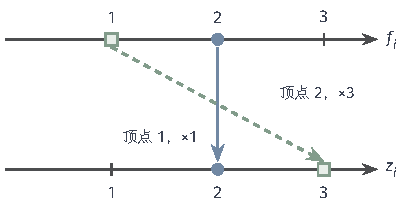
\includegraphics{figures/03-graphs/05-matrices-and-spectra/tikz/ncut-coordinate-order/figure.pdf}
  \caption{度数缩放可能改变顶点的排序先后。圆点对应度数$d_1=1$的顶点，方点对应度数$d_2=9$的顶点。按$z_i=\sqrt{d_i}\,f_i$转换到下轴时，方点坐标从$1$放大为$3$并反超圆点。阈值扫描必须使用上方的还原坐标$f_i$轴。}
  \label{fig:graph-ncut-coordinate-order}
\end{BookInlineFigure}

在单位权四点路径$1\!-\!2\!-\!3\!-\!4$上，各点度数为$(1,2,2,1)$，还原后的特征向量为$\bm f=(2,1,-1,-2)^\top$，按$f_i$从大到小排序仍为$1,2,3,4$。三个前缀候选切口的指标如下：切下$\{1\}$时割权为$1$、两侧体积为$1$和$5$，$\operatorname{NCut}=1\times(1+\frac15)=\frac65$；切断中间边得$\{1,2\}$时割权为$1$、两侧体积均为$3$，$\operatorname{NCut}=1\times(\frac13+\frac13)=\frac23$；切出$\{1,2,3\}$时$\operatorname{NCut}=\frac65$。算法返回中间割$\{1,2\}\mid\{3,4\}$，其NCut值$\frac23$夹在松弛下界$\mu_2=\frac12$之上。

\subsection{算法分析}
\label{sec:graph-ncut-guarantee}

记全图所有合法二分中的NCut真实最小值为$\operatorname{OPT}_N$，算法~\ref{alg:graph-ncut-sweep}扫描输出的划分为$S_N$。与RatioCut类似，松弛值$\mu_2$给出下界，扫描结果给出可行上界：
\begin{equation}
\label{eq:graph-ncut-bounds}
\mu_2(\mathcal L)\leq\operatorname{OPT}_N\leq\operatorname{NCut}(S_N,\bar S_N).
\end{equation}

NCut的松弛与阈值扫描使用的算子和坐标，与Cheeger不等式上界证明中的对象相同。由此可以得到不显式含最大度或最小度的目标值上界。下面分别核对目标函数、松弛方向和候选割之间的关系。

\paragraph{1. 目标函数同源：NCut与导通率$\phi(S)$仅差至多$2$倍}

对任意非空真子集$S\subsetneq V$，设两侧体积分别为$a=\operatorname{vol}(S)$和$b=\operatorname{vol}(\bar S)$，且不妨设$a\leq b$（即$a=\min\{\operatorname{vol}(S),\operatorname{vol}(\bar S)\}$）。对比定义~\ref{def:graph-conductance}与定义~\ref{def:graph-ncut}：
\[
\operatorname{NCut}(S,\bar S)
=\frac{c(S,\bar S)}{a}+\frac{c(S,\bar S)}{b}
=\frac{c(S,\bar S)}{a}\left(1+\frac{a}{b}\right)
=\phi(S)\left(1+\frac{a}{b}\right).
\]
由于$0<a\leq b$，比值$\frac{a}{b}$必定落在$(0,1]$内，故$1<\left(1+\frac{a}{b}\right)\leq 2$。因此，对图上的任何一个割，NCut与导通率$\phi(S)$都被锁定在常数$2$倍以内：
\begin{equation}
\label{eq:ncut-conductance-equivalence}
\phi(S)\leq\operatorname{NCut}(S,\bar S)\leq 2\phi(S).
\end{equation}

\paragraph{2. 谱松弛与扫描顺序完全一致}

对比式~\eqref{eq:graph-normalized-variational-cut}与式~\eqref{eq:ncut-spectral-relaxation}可以看到：Cheeger不等式所用的特征值$\mu_2(\mathcal L)$，与NCut连续谱松弛得到的下界$\mu_2(\mathcal L)$是\emph{同一个特征值}；而且第~\ref{sec:graph-cheeger-sweep}小节证明Cheeger上界时所扫描的特征向量$\bm f=\bm D^{-1/2}\bm z_2$，与算法~\ref{alg:graph-ncut-sweep}第三步排序所用的还原向量$\bm f=\bm D^{-1/2}\bm z_2$也是\emph{同一个向量}。换言之，NCut阈值扫描所考察的至多$|V_+|-1$个阈值前缀候选集，与Cheeger不等式上界证明所考察的前缀候选集完全相同。

\paragraph{3. 由Cheeger不等式直接导出NCut的性能保证}

由第~\ref{sec:graph-cheeger-sweep}小节的证明，同一批前缀候选中存在$S_\phi$使$\phi(S_\phi)\leq\sqrt{2\mu_2}$。算法在这些候选中最小化NCut，故$\operatorname{NCut}(S_N,\bar S_N)\leq\operatorname{NCut}(S_\phi,\bar S_\phi)$。再用$\operatorname{NCut}(S_\phi,\bar S_\phi)\leq2\phi(S_\phi)$和松弛下界$\mu_2\leq\operatorname{OPT}_N$，得到
\begin{equation}
\label{eq:graph-ncut-sweep-bound}
\begin{aligned}
\mu_2(\mathcal L)
&\leq \operatorname{OPT}_N
\leq \operatorname{NCut}(S_N,\bar S_N)
\leq \operatorname{NCut}(S_\phi,\bar S_\phi) \\
&\leq 2\phi(S_\phi)
\leq 2\sqrt{2\mu_2(\mathcal L)}
\leq 2\sqrt{2\operatorname{OPT}_N}.
\end{aligned}
\end{equation}

式~\eqref{eq:graph-ncut-sweep-bound}给出平方根形式的目标值保证。若$\operatorname{OPT}_N>0$，相除得到的近似因子为$2\sqrt{2/\operatorname{OPT}_N}$，并非常数；因此不能由此推断NCut在所有任务上优于RatioCut。得到准确谱向量后，排序与增量扫描共需$O(n\log n+m)$时间，特征向量求解的成本须另计。对于近似特征向量，还需根据其Rayleigh商和正交误差重新核对保证。

\begin{BookInlineFigure}
  \centering
  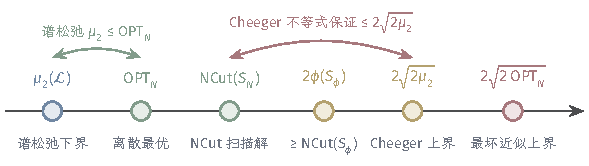
\includegraphics[width=99.713mm]{figures/03-graphs/05-matrices-and-spectra/tikz/ncut-sweep-and-cheeger-chain/figure.pdf}
  \caption{NCut谱划分与Cheeger不等式结合形成的双向近似保证链。左侧由连续谱松弛给出下界$\mu_2(\mathcal L)\leq\operatorname{OPT}_N$，右侧由Cheeger阈值扫描上界保证扫描输出解$S_N$满足$\operatorname{NCut}(S_N)\leq 2\sqrt{2\mu_2}\leq 2\sqrt{2\operatorname{OPT}_N}$。}
  \label{fig:graph-ncut-sweep-guarantee}
\end{BookInlineFigure}

\section{谱划分方法的比较}
\label{sec:graph-spectral-partition-comparison}

RatioCut与NCut同属基于拉普拉斯二次型松弛的谱划分方法，两者的算法骨架高度一致，核心区别仅在于\emph{如何定义子图的规模}：RatioCut按“顶点个数$|A|$”计规模，追求两侧节点数量的均衡；NCut按“度数总和（体积$\operatorname{vol}(A)$）”计规模，衡量跨割权相对于两侧总度数的比例。表~\ref{tab:ratiocut-vs-ncut}汇总了两种方法在各个环节的一一对应关系。

\begin{table}[!htb]
\centering
\caption{RatioCut与NCut谱划分方法的核心要素对比。}
\label{tab:ratiocut-vs-ncut}
\footnotesize
\begin{tabular}{lll}
\toprule
对比维度 & RatioCut（比例割） & NCut（归一化割）\\
\midrule
均衡目标 & 节点个数$|A|,|B|$均衡 & 度体积$\operatorname{vol}(A),\operatorname{vol}(B)$均衡\\
目标函数 & $c(A,B)\bigl(\frac{1}{|A|}+\frac{1}{|B|}\bigr)$ & $c(A,B)\bigl(\frac{1}{\operatorname{vol}(A)}+\frac{1}{\operatorname{vol}(B)}\bigr)$\\
两值向量$f_i$ & $\sqrt{|B|/|A|},-\sqrt{|A|/|B|}$ & 式~\eqref{eq:ncut-indicator-vector}的两值\\
等价Rayleigh商 & $\dfrac{\bm f^\top\bm L\bm f}{\bm f^\top\bm f}$ & $\dfrac{\bm f^\top\bm L\bm f}{\bm f^\top\bm D\bm f}$\\
松弛算子 & 组合拉普拉斯$\bm L=\bm D-\bm W$ & 对称归一化$\mathcal L=\bm D^{-1/2}\bm L\bm D^{-1/2}$\\
下界与排序 & $\lambda_2(\bm L)$，按$\bm v_2$排序 & $\mu_2(\mathcal L)$，按$\bm f=\bm D^{-1/2}\bm z_2$排序\\
Cheeger保证 & 需另行给出相应尺度的界 & $\operatorname{NCut}(S_N)\leq 2\sqrt{2\operatorname{OPT}_N}$\\
\bottomrule
\end{tabular}
\end{table}

在正则图上，两种目标成比例；度数不完全相同时，即使差异较小，也不能保证最优划分一致。下面通过一个具体的四点加权路径算例直观展示这一分歧。

\paragraph{加权路径上的最优割分歧}

考虑图~\ref{fig:graph-partition-weighted-path}所示的四顶点路径$1\!-\!2\!-\!3\!-\!4$，将其三条边的权重设为中间重、两端轻：$w_{12}=1$，$w_{23}=2$，$w_{34}=1$。由此算出四个顶点的加权度依次为$d_1=1,d_2=3,d_3=3,d_4=1$，全图总体积为$\operatorname{vol}(V)=8$。

\begin{BookInlineFigure}
  \centering
  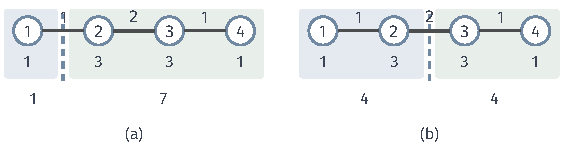
\includegraphics{figures/03-graphs/05-matrices-and-spectra/tikz/partition-weighted-path/figure.pdf}
  \caption{加权路径（边权$1,2,1$）上的两个关键候选割。(a) 切下左端点$1$：只切断权重为$1$的端边，两侧顶点数为$1$对$3$，两侧体积为$1$对$7$。(b) 沿中间边切开：需切断权重为$2$的粗边，但两侧顶点数（$2$对$2$）与体积（$4$对$4$）均相等。顶点下方标注加权度。}
  \label{fig:graph-partition-weighted-path}
\end{BookInlineFigure}

我们重点比较图~\ref{fig:graph-partition-weighted-path}标出的两种切法：
\begin{enumerate}
\item \emph{候选一：切下低度端点$\{1\}\mid\{2,3,4\}$}（图a，与切下右端点$\{4\}\mid\{1,2,3\}$对称）。这一刀避开了中间权重为$2$的粗边，只切断权重为$1$的轻边$12$，故割权$c=1$。两侧的节点个数为$|A|=1,|B|=3$，而两侧的体积则悬殊为$\operatorname{vol}(A)=1,\operatorname{vol}(B)=7$。代入两个目标函数：
\[
\begin{aligned}
  \operatorname{RatioCut}(\{1\}) &= 1\times\left(\frac{1}{1}+\frac{1}{3}\right) = \frac{4}{3}\approx 1.333, \\
  \operatorname{NCut}(\{1\}) &= 1\times\left(\frac{1}{1}+\frac{1}{7}\right) = \frac{8}{7}\approx 1.143.
\end{aligned}
\]
\item \emph{候选二：切断中间重边$\{1,2\}\mid\{3,4\}$}（图b）。这一刀直接切断权重为$2$的中间边$23$，割权升至$c=2$，但换来了两侧规模相等——两侧节点个数为$2$对$2$，两侧体积均为$1+3=4$。代入两个目标函数：
\[
  \operatorname{RatioCut}(\{1,2\}) = 2\times\left(\frac{1}{2}+\frac{1}{2}\right) = 2,
  \qquad
  \operatorname{NCut}(\{1,2\}) = 2\times\left(\frac{1}{4}+\frac{1}{4}\right) = 1.
\]
\end{enumerate}

至于其余非空二分（如将两端点合为一组的$\{1,4\}\mid\{2,3\}$，或奇偶交错的$\{1,3\}\mid\{2,4\}$），它们同时切断了两条或三条边，割权不低于$2$且规模不比中间割更优。图~\ref{fig:graph-comparison-four-bipartitions}与下表展示了四类代表性二分；下表还列出了切下内部顶点的第五类，从而覆盖所有非空二分（对称情形合并）的结构与指标：

\begin{BookInlineFigure}
  \centering
  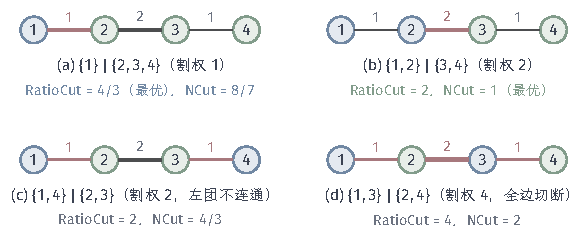
\includegraphics[width=98.316mm]{figures/03-graphs/05-matrices-and-spectra/tikz/comparison-four-bipartitions/figure.pdf}
  \caption{加权路径（边权$1,2,1$）的四类非空二分结构对比。蓝色与绿色区分两侧子集，红色边表示被切断的跨割边。(a) 切下单个端点，RatioCut达到全局最小$4/3$；(b) 切断中间重边，NCut达到全局最小$1$；(c) 两端点合并为一侧，同时切断两条端边且左侧不连通；(d) 奇偶交错分组，三条边全部被切断。}
  \label{fig:graph-comparison-four-bipartitions}
\end{BookInlineFigure}
\begin{center}
\small
\setlength{\tabcolsep}{4pt}
\begin{tabular}{lccccc}
\toprule
候选划分 & 割权$c$ & 节点数 & 两侧体积 & RatioCut & NCut\\
\midrule
$\{1\}\mid\{2,3,4\}$ & $1$ & $1,3$ & $1,7$ & $\mathbf{4/3}$ & $8/7$\\
$\{1,2\}\mid\{3,4\}$ & $2$ & $2,2$ & $4,4$ & $2$ & $\mathbf{1}$\\
$\{2\}\mid\{1,3,4\}$ & $3$ & $1,3$ & $3,5$ & $4$ & $8/5$\\
$\{1,4\}\mid\{2,3\}$ & $2$ & $2,2$ & $2,6$ & $2$ & $4/3$\\
$\{1,3\}\mid\{2,4\}$ & $4$ & $2,2$ & $4,4$ & $4$ & $2$\\
\bottomrule
\end{tabular}
\end{center}

枚举全部二分后，RatioCut的最小值为$4/3$，由两种端点割取得；NCut的最小值为$1$，由中间割取得。端点割将割权从$2$减为$1$，足以抵消RatioCut中的顶点数失衡代价；在NCut中，端点仅占总体积的$1/8$，其代价$8/7$仍大于中间割的$1$。这一差异来自两个目标采用的规模度量。

\paragraph{正则图上的统一性与实践选择建议}

当图是加权度恒为常数$d>0$的$d$正则图时，任意子集$A$的体积恒等于节点数的$d$倍：$\operatorname{vol}(A)=d|A|$。此时NCut与RatioCut严格成正比：
\[
\operatorname{NCut}(A,B)
=c(A,B)\left(\frac{1}{d|A|}+\frac{1}{d|B|}\right)
=\frac{1}{d}\operatorname{RatioCut}(A,B),
\]
对称归一化拉普拉斯也简化为$\mathcal L=\frac{1}{d}\bm L$，两种离散目标具有相同的最优划分。若选择相同的特征方向并使用一致的并列处理规则，谱扫描的排序与结果也相同；重特征值或多个最优切口可能使不同实现返回不同划分。

选择目标应依据任务如何衡量规模。若每个顶点代表等量负载，可以考虑RatioCut；若关心每侧跨组连接占总连接量的比例，可以考虑NCut。二者都是软性的均衡目标，均不保证指定的组大小或内部密度。若任务要求严格等分，应另加规模约束，并重新分析算法和保证。

\section{本章小结}
\label{sec:graph-spectral-partition-summary}

组合拉普拉斯的第二小特征值$\lambda_2$衡量连通图连得有多紧。它不低于点连通度和边连通度（对简单无权非完全图），Fiedler向量的非负一侧在连通图上保持连通。但$\lambda_2$会随边权整体放大而增大，跨图比较时需要消除尺度。

归一化拉普拉斯的第二小特征值$\mu_2$用度加权长度替代普通长度。Cheeger不等式把$\mu_2$与最小导通率$\phi_*$从两侧绑在一起：下界$\mu_2/2\leq\phi_*$说明图中不存在太稀疏的平衡割，上界$\phi_*\leq\sqrt{2\mu_2}$提供了一个构造性的搜索——按特征方向排序并扫描阈值，其中至少一个割满足导通率保证。超立方体实现了下界等号，长环展示了上界中平方根尺度的必要性。

实际分组只给顶点两种值。RatioCut用顶点数计量组规模，松弛为$\lambda_2$的变分问题。NCut用度的总和计量，松弛为$\mu_2$的变分问题。两者的流程相同：求特征向量、排序、逐阈值扫描、按原目标选出最优候选。松弛值是离散最优值的下界，扫描候选给出上界，两者合在一起为分组质量提供可核验的区间。

这些步骤反复用到拉普拉斯的二次型。下一章研究怎样用更少的边同时近似保留所有顶点方向上的能量，并将这种稀疏近似用于方程求解。

